\ifx\allfiles\undefined
\documentclass[12pt, a4paper,oneside, UTF8]{ctexbook}
\usepackage[dvipsnames]{xcolor}
\usepackage{mathtools}   % 数学公式
\usepackage{amsthm}    % 定理环境
\usepackage{amssymb}   % 更多公式符号
\usepackage{graphicx}  % 插图
%\usepackage{mathrsfs}  % 数学字体
%\usepackage{newtxtext,newtxmath}
%\usepackage{arev}
\usepackage{kmath,kerkis}
\usepackage{newtxtext}
\usepackage{bbm}
\usepackage{enumitem}  % 列表
\usepackage{geometry}  % 页面调整
%\usepackage{unicode-math}
\usepackage[colorlinks,linkcolor=black]{hyperref}

\usepackage{wrapfig}


\usepackage{ulem}	   % 用于更多的下划线格式,
					   % \uline{}下划线,\uuline{}双下划线,\uwave{}下划波浪线,\sout{}中间删除线,\xout{}斜删除线
					   % \dashuline{}下划虚线,\dotuline{}文字底部加点


\graphicspath{ {flg/},{../flg/}, {config/}, {../config/} }  % 配置图形文件检索目录
\linespread{1.5} % 行高

% 页码设置
\geometry{top=25.4mm,bottom=25.4mm,left=20mm,right=20mm,headheight=2.17cm,headsep=4mm,footskip=12mm}

% 设置列表环境的上下间距
\setenumerate[1]{itemsep=5pt,partopsep=0pt,parsep=\parskip,topsep=5pt}
\setitemize[1]{itemsep=5pt,partopsep=0pt,parsep=\parskip,topsep=5pt}
\setdescription{itemsep=5pt,partopsep=0pt,parsep=\parskip,topsep=5pt}

% 定理环境
% ########## 定理环境 start ####################################
\theoremstyle{definition}
\newtheorem{defn}{\indent 定义}[section]

\newtheorem{lemma}{\indent 引理}[section]    % 引理 定理 推论 准则 共用一个编号计数
\newtheorem{thm}[lemma]{\indent 定理}
\newtheorem{corollary}[lemma]{\indent 推论}
\newtheorem{criterion}[lemma]{\indent 准则}

\newtheorem{proposition}{\indent 命题}[section]
\newtheorem{example}{\indent \color{SeaGreen}{例}}[section] % 绿色文字的 例 ,不需要就去除\color{SeaGreen}{}
\newtheorem*{rmk}{\indent \color{red}{注}}

% 两种方式定义中文的 证明 和 解 的环境:
% 缺点:\qedhere 命令将会失效【技术有限,暂时无法解决】
\renewenvironment{proof}{\par\textbf{证明.}\;}{\qed\par}
\newenvironment{solution}{\par{\textbf{解.}}\;}{\qed\par}

% 缺点:\bf 是过时命令,可以用 textb f等替代,但编译会有关于字体的警告,不过不影响使用【技术有限,暂时无法解决】
%\renewcommand{\proofname}{\indent\bf 证明}
%\newenvironment{solution}{\begin{proof}[\indent\bf 解]}{\end{proof}}
% ######### 定理环境 end  #####################################

% ↓↓↓↓↓↓↓↓↓↓↓↓↓↓↓↓↓ 以下是自定义的命令  ↓↓↓↓↓↓↓↓↓↓↓↓↓↓↓↓

% 用于调整表格的高度  使用 \hline\xrowht{25pt}
\newcommand{\xrowht}[2][0]{\addstackgap[.5\dimexpr#2\relax]{\vphantom{#1}}}

% 表格环境内长内容换行
\newcommand{\tabincell}[2]{\begin{tabular}{@{}#1@{}}#2\end{tabular}}

% 使用\linespread{1.5} 之后 cases 环境的行高也会改变,重新定义一个 ca 环境可以自动控制 cases 环境行高
\newenvironment{ca}[1][1]{\linespread{#1} \selectfont \begin{cases}}{\end{cases}}
% 和上面一样
\newenvironment{vx}[1][1]{\linespread{#1} \selectfont \begin{vmatrix}}{\end{vmatrix}}

\def\d{\textup{d}} % 直立体 d 用于微分符号 dx
\def\R{\mathbb{R}} % 实数域
\def\N{\mathbb{N}} % 自然数域
\def\C{\mathbb{C}} % 复数域
\def\Z{\mathbb{Z}} % 整数环
\def\Q{\mathbb{Q}} % 有理数域
\newcommand{\bs}[1]{\boldsymbol{#1}}    % 加粗,常用于向量
\newcommand{\ora}[1]{\overrightarrow{#1}} % 向量

% 数学 平行 符号
\newcommand{\pll}{\kern 0.56em/\kern -0.8em /\kern 0.56em}

% 用于空行\myspace{1} 表示空一行 填 2 表示空两行  
\newcommand{\myspace}[1]{\par\vspace{#1\baselineskip}}

%s.t. 用\st就能打出s.t.
\DeclareMathOperator{\st}{s.t.}

%罗马数字 \rmnum{}是小写罗马数字, \Rmnum{}是大写罗马数字
\makeatletter
\newcommand{\rmnum}[1]{\romannumeral #1}
\newcommand{\Rmnum}[1]{\expandafter@slowromancap\romannumeral #1@}
\makeatother
\begin{document}
	% \title{{\Huge{\textbf{$Functional \,\, Analysis$}}}\footnote{参考书籍:\\
			\hspace*{4em} \textbf{《Linear and Nonlinear Functional Analysis with Applications》 -- Philippe G. Ciarlet} \\
			\hspace*{4em} \textbf{《Real  Analysis -- Modern Techniques and Their Applications》 -- Gerald  B.  Folland} \\
			\hspace*{4em} \textbf{《Functional Analysis -- Introduction to Further Topics in Analysis》 -- Elias M. Stein} \\
			\hspace*{4em} \textbf{《泛函分析讲义》 -- 张恭庆、林源渠} 
			}}
\author{$-TW-$}
\date{\today}
\maketitle                   % 在单独的标题页上生成一个标题

\thispagestyle{empty}        % 前言页面不使用页码
\begin{center}
	\Huge\textbf{序}
\end{center}


\vspace*{3em}
\begin{center}
	\large{\textbf{天道几何,万品流形先自守;}}\\
	
	\large{\textbf{变分无限,孤心测度有同伦。}}
\end{center}

\vspace*{3em}
\begin{flushright}
	\begin{tabular}{c}
		\today \\ \small{\textbf{长夜伴浪破晓梦,梦晓破浪伴夜长}}
	\end{tabular}
\end{flushright}


\newpage                      % 新的一页
\pagestyle{plain}             % 设置页眉和页脚的排版方式(plain:页眉是空的,页脚只包含一个居中的页码)
\setcounter{page}{1}          % 重新定义页码从第一页开始
\pagenumbering{Roman}         % 使用大写的罗马数字作为页码
\tableofcontents              % 生成目录

\newpage                      % 以下是正文
\pagestyle{plain}
\setcounter{page}{1}          % 使用阿拉伯数字作为页码
\pagenumbering{arabic}
\setcounter{chapter}{0}    % 设置 -1 可作为第零章绪论从第零章开始 
	\else
	\fi
	%  ############################ 正文部分
\chapter{度量空间}

\section{$L^p$ 空间为赋范向量空间}
\begin{center}
	回顾实分析中对\textbf{范数}、\textbf{度量}及\textbf{$L^p$ 空间}的定义.
\end{center}
	
\subsection{范数,度量}
	下面给出\textbf{范数}和\textbf{度量}的严格定义.
	\begin{defn}\label{def 1.1.1}
		Let $X$ be a vector space over field $\mathbb{K}$, a \underline{\textcolor{blue}{\textbf{norm}}} is a function:
		\begin{align}
			X &\longrightarrow \R_{\geq 0} \\
			f &\longmapsto \Vert f \Vert
		\end{align}
		satisfying the following properties:
		\begin{enumerate}
			\item[(\rmnum{1})]$\Vert f \Vert \geq 0$, $\forall f \in X$. \hspace*{3em} ($\Vert f \Vert = 0 \,\, \Leftrightarrow \,\, f = 0 \,\, a.e.$)
			
			\item[(\rmnum{2})]$\Vert af \Vert = \left| a \right| \Vert f \Vert$, $\forall a \in \mathbb{K}, f \in X$.
			
			\item[(\rmnum{3})]$\Vert f + g \Vert \leq \Vert f \Vert + \Vert g \Vert$, $\forall f , g \in X$.
		\end{enumerate}
		
		\vspace{2em}
		\begin{rmk}
			\begin{itemize}
				\item (\rmnum{1})中的“$\Vert f \Vert = 0 \,\, \Leftrightarrow \,\, f = 0 \,\, a.e.$”的\textbf{“a.e.”}是对于$X$ 取函数空间时的条件,在实分析的取等条件中基本为默认叙述,在后续定义中往往省略. 在对$\mathcal{L}^p$ 空间的定义 (\textbf{定义 \ref{def 1.1.3}})中可以看到其合理性.
				
				\vspace{1em}
				
				\item \textbf{范数}实际上是对$\R^n$ 空间中\textbf{“与原点之间的距离”}这一概念的推广. 将函数视作向量,则其范数即为到原点的距离,即\textbf{模长}.
				
				\vspace{1em}
				
				\item 若一个\textbf{线性空间}$X$ 上配备了一个\textbf{范数},则称其为\textcolor{blue}{\textbf{赋范向量空间 (赋范线性空间)}}.
			\end{itemize}
		\end{rmk}
	\end{defn}
	
	\newpage
	将函数视作向量,就有其\textbf{到原点的距离}为\textbf{范数}. 但若是想要衡量\textbf{任意两个函数之间的距离},则需要引入下面\textbf{度量}的概念.
	\begin{defn}\label{def 1.1.2}
		A \underline{\textcolor{blue}{\textbf{metric}}} on $X$ is a map
		\begin{align}
			\rho : X \times X &\longrightarrow \R_{\geq 0} \\
			(x , y) &\longmapsto \rho(x , y)
		\end{align}
		satisfying
		\begin{enumerate}
			\item[(\rmnum{1})]$\rho(x,  y) \geq 0$, $\forall x , y \in X$. \hspace*{3em} ($\rho(x , y) = 0 \,\, \Leftrightarrow \,\, x = y$)
			
			\item[(\rmnum{2})]$\rho(x , y) = \rho(y , x)$, $\forall x , y \in X$.
			
			\item[(\rmnum{3})]$\rho(x , y) + \rho(y , z) \geq \rho(x , z)$, $\forall x , y , z \in X$.
		\end{enumerate}
		
		\vspace{2em}
		\begin{rmk}
			\begin{itemize}
				\item 若$X$ 为函数空间,则 (\rmnum{1})中“$\rho(x , y) = 0$”等价条件默认为“$x = y \,\, a.e.$”.
				
				\vspace{1em}
				
				\item \textbf{度量}可看作将两个函数 (向量)的起点均平移至原点后,其两个终点之间的\textbf{距离}.
			\end{itemize}
		\end{rmk}
	\end{defn}

\vspace{4em}
\subsection{$L^p$ Space}
\paragraph{$L^p \,\, Space$}
	下面给出\textbf{$L^p$ 空间}的定义.
	\begin{defn}\label{def 1.1.3}
		For any measure space $(X , \mathcal{M} , \mu)$, define the \underline{\textcolor{blue}{\textbf{$L^p \,\, Space \,\, L^{p}(X)$}}} on $X$ ($1 \leq p < \infty$)
		\begin{align}
			L^{p}(X) &= \left\{ f \in \mathcal{M} \mid \int_{X}{\left| f \right|^p d \mu} < \infty \right\} , \,\, \forall 1 \leq p < \infty\\
			L^{\infty}(X) &= \left\{ f \in \mathcal{M} \, \Big| \, \inf{\left\{ C \geq 0 \mid \left| f \right| \leq C \,\, a.e. \right\}} < \infty \right\}
		\end{align}
		
		\vspace{2em}
		\begin{rmk}
			与$L^1$ 空间 (即可积函数构成的空间)类似, 后面我们考虑的$L^{p}(X)$ 空间事实上为\textbf{几乎处处相等}意义下的完全剩余系, 即在$L^{p}(X)$ 空间上定义一个等价关系$\sim$:
			\begin{center}
				$f \sim g \,\, \Leftrightarrow \,\, f = g \,\, a.e.$
			\end{center}
			此时再令$L^{p}(X)$ 空间模去该等价关系$\sim$, 即
			\begin{center}
				$L^{p}(X) \coloneqq L^{p}(X) / \sim$
			\end{center}
		\end{rmk}
	\end{defn}

\newpage

\paragraph{$L^p$ 范数}
	在$L^{p}$ 空间上, 我们来定义\textbf{$L^p$ 范数}.
	\begin{defn}\label{def 1.1.4}
		Measure space $(X , \mathcal{M} , \mu)$. For any function $f \in L^{p}(X)$, define the \underline{\textcolor{blue}{\textbf{$L^p$ norm}}} of $f$
		\begin{align}
			\Vert f \Vert_{p} &= \left( \int_{X}{\left| f \right|^p d\mu} \right)^{\frac{1}{p}} , \,\, \forall 1 \leq p < \infty \\
			\Vert f \Vert_\infty &= \inf{\left\{ C \geq 0 \mid \left| f \right| \leq C \,\, a.e. \right\}}
		\end{align}
		
		\vspace{2em}
		\begin{rmk}
			\begin{itemize}
				\item 不难得到$L^\infty$ 范数的\textbf{等价定义}为
				\begin{align}
					\Vert f \Vert_\infty = \sup{\left\{ C \geq 0 \mid \mu(\left| f \right| > C ) > 0 \right\}}
				\end{align}
			
				\vspace{1em}
				
				\item 为了说明上述定义是well-defined, 我们需要验证其满足\textbf{范数的三条公理 (Def \ref{def 1.1.1})}. \\
				其中前面两条 (正定性、绝对齐性)是显然的, 而对于三角不等式, 我们需要用到后续证明的\textbf{Minkowski Inequality (Thm \ref{thm 1.1.4})}.
			\end{itemize}
		\end{rmk}
	\end{defn}
	
	\vspace{4em}
	事实上, 在证明了\textbf{Minkowski Inequality (Thm \ref{thm 1.1.4})} 后, 我们还可得到$L^{p}(X)$ 为\textbf{线性空间}, 从而证明$(L^{p}(X) , \,\, \Vert \cdot \Vert_p)$ 为\textbf{赋范向量空间}. 下面我们的证明思路如下:
	\begin{center}
		\textbf{Young Inequality} $\,\, \Rightarrow \,\,$ \textbf{H\"{o}lder Inequality} $\,\, \Rightarrow \,\,$ \textbf{Minkowski Inequality}
	\end{center}

\newpage
\subsection{Young Inequality}
	为了证明\textbf{H\"{o}lder不等式}, 先来给出\textbf{Young不等式}, 可视作一条\textbf{均值不等式的加权推广}.
	\begin{thm}\label{thm 1.1.1}
		\textbf{Young Inequality}. \\
		Suppose $p , q > 0$ and $\frac{1}{p} + \frac{1}{q} = 1$. Then for $\forall a , b \geq 0$, $\st$
		\begin{align}
			ab \leq \frac{1}{p} a^p + \frac{1}{q} b^q
		\end{align}
		
		\vspace{2em}
		\begin{rmk}
			\textbf{Young不等式}可视作一条均值不等式 (几何平均数$\leq$ 平方平均数)的\textbf{加权推广}, 即
			\begin{center}
				$\sqrt{ab} \leq \sqrt{\frac{a^2 + b^2}{2}}$
			\end{center}
		\end{rmk}
		
		\vspace{2em}
		\begin{proof}
			(利用\textbf{指数函数的凸性}及\textbf{Jensen Inequality}). \\
			It's trivial when $a = 0$ or $b = 0$. 不妨设$a , b \neq 0$, 即$a , b > 0$. \\
			Since $f(x) = e^x$ is convex, $\frac{1}{p} + \frac{1}{q} = 1$, then by \textbf{Jensen Inequality},
			\begin{align}
				e^{\frac{x}{p} + \frac{y}{q}} \leq \frac{1}{p} e^x + \frac{1}{q} e^y , \,\, \forall x , y \in \R
			\end{align}
			Let $x = \log{a^p}$, $y = \log{b^q}$, $\forall a , b > 0$, then
			\begin{align}
				ab \leq \frac{a^p}{p} + \frac{b^q}{q} , \,\, \forall a , b > 0
			\end{align}
		\end{proof}
	\end{thm}
	
	\vspace{4em}
	下面给出一条推论, 将用于\textbf{H\"{o}lder Inequality} 的证明中.
	\begin{corollary}\label{cor 1.1.2}
		Suppose $p , q > 0$ and $\frac{1}{p} + \frac{1}{q} = 1$. Then for $\forall f \in L^p , g \in L^q$, $\st$
		\begin{align}
			\int{\left| f g \right|} \leq \frac{1}{p} \int{\left| f \right|^p} + \frac{1}{q} \int{\left| g \right|^q}
		\end{align}
		
		\vspace{2em}
		\begin{proof}
			By \textbf{Young Inequality (Thm \ref{thm 1.1.1})}, 逐点均有
			\begin{align}
				\left| fg \right| (x) \leq \frac{1}{p} \left| f \right|^p (x) + \frac{1}{q} \left| g \right|^q (x) , \,\, \forall x \in X
			\end{align}
			积分, 得
			\begin{align}
				\int{\left| f g \right|} \leq \frac{1}{p} \int{\left| f \right|^p} + \frac{1}{q} \int{\left| g \right|^q}
			\end{align}
		\end{proof}
	\end{corollary}

\newpage
\subsection{H\"{o}lder Inequality}
 	下面给出\textbf{二元情形下的H\"{o}lder不等式}.
 	\begin{thm}\label{thm 1.1.3}
 		\textbf{H\"{o}lder Inequality}. \\
 		Suppose $1 < p , q < \infty$ and $\frac{1}{p} + \frac{1}{q} = 1$. Then $\forall f \in L^{p} , g \in L^q$, $\st$ $fg \in L^1$ and
 		\begin{align}
 			\Vert fg \Vert_1 \leq \Vert f \Vert_p \cdot \Vert g \Vert_q
 		\end{align}
 		
 		\vspace{4em}
 		\begin{proof}
 			It's trivial when $\Vert f \Vert_p = 0$ or $\Vert g \Vert_q = 0$. 不妨设$\Vert f \Vert_p, \,\, \Vert g \Vert_q \neq 0$. \\
 			不妨设$\Vert f \Vert_p = \Vert g \Vert_q = 1$. (Otherwise we can let $\widetilde{f} = \frac{f}{\Vert f \Vert_p}$ and $\widetilde{g} = \frac{g}{\Vert g \Vert_q}$) \\
 			Then by \textbf{Young Inequality (Cor \ref{cor 1.1.2})},
 			\begin{align}
 				\Vert fg \Vert_1 
 				= \int{\left| fg \right|}
 				&\leq \frac{1}{p} \int{\left| f \right|^p} + \frac{1}{q} \int{\left| g \right|^q} \\
 				&= \frac{1}{p} \Vert f \Vert_{p}^{p} + \frac{1}{q} \Vert g \Vert_{q}^{q} \\
 				&= \frac{1}{p} + \frac{1}{q} \\
 				&= 1 
 				= \Vert f \Vert_p \cdot \Vert g \Vert_q
 			\end{align}
 		\end{proof}
 	\end{thm}
 
 \newpage
 
 \subsection{Minkowski Inequality}
 	下面给出\textbf{Minkowski不等式}的内容, 它说明了我们所定义的$L^p$ 范数$\Vert \cdot \Vert_p$ (Def \ref{def 1.1.4}) 的合理性, 并且可以推出$L^p$ 空间为\textbf{线性空间}, 从而得到$(L^p(X) , \,\, \Vert \cdot \Vert_p)$ 为\textbf{赋范向量空间}.
 	\begin{thm}\label{thm 1.1.4}
 		\textbf{Minkowski Inequality}. \\
 		Suppose $1 \leq p < \infty$. Then for $\forall f , g \in L^p$, $\st$
 		\begin{align}
 			\Vert f + g \Vert_p \leq \Vert f \Vert_p + \Vert g \Vert_p
 		\end{align}
 		
 		\vspace{4em}
 		\begin{proof}
 			$\forall f , g \in L^p$, we have
 			\begin{align}
 				\Vert f + g \Vert_{p}^p 
 				= \int{\left| f + g \right|^p} 
 				&= \int{\left| f + g \right| \cdot \left| f + g \right|^{p - 1}} \\
 				&\leq \int{\left| f \right| \cdot \left| f + g \right|^{p - 1}} + \int{\left| g \right| \cdot \left| f + g \right|^{p - 1}}
 			\end{align}
 			By \textbf{H\"{o}lder Inequality (Thm \ref{thm 1.1.3})},
 			\begin{align}
 				\int{\left| f \right| \cdot \left| f + g \right|^{p - 1}}
 				= \Vert \left| f \right| \cdot \left| f + g \right|^{p - 1} \Vert_{1} 
 				\leq \left( \int{\left| f \right|^p} \right)^{\frac{1}{p}} \cdot \left( \int{\left| f + g \right|^{(p - 1) \cdot q}} \right)^{\frac{1}{q}}
 			\end{align}
 			where $\frac{1}{p} + \frac{1}{q} = 1$. Thus $q = \frac{p}{p - 1}, (p - 1) q = p$, we have
 			\begin{align}
 				\int{\left| f \right| \cdot \left| f + g \right|^{p - 1}}
 				\leq \left( \int{\left| f \right|^p} \right)^{\frac{1}{p}} \cdot \left( \int{\left| f + g \right|^{p}} \right)^{\frac{p - 1}{p}}
 				= \Vert f \Vert_{p} \cdot \Vert f + g \Vert_{p}^{p - 1}
 			\end{align}
 			Similarly, we get
 			\begin{align}
 				\int{\left| g \right| \cdot \left| f + g \right|^{p - 1}}
 				\leq \left( \int{\left| g \right|^p} \right)^{\frac{1}{p}} \cdot \left( \int{\left| f + g \right|^{p}} \right)^{\frac{p - 1}{p}}
 				= \Vert g \Vert_{p} \cdot \Vert f + g \Vert_{p}^{p - 1}
 			\end{align}	
 			Therefore,
 			\begin{align}
 				\Vert f + g \Vert_{p}^{p} 
 				&\leq \int{\left| f \right| \cdot \left| f + g \right|^{p - 1}} + \int{\left| g \right| \cdot \left| f + g \right|^{p - 1}} \\
 				&\leq \left( \Vert f \Vert_{p} + \Vert g \Vert_{p} \right) \cdot \Vert f + g \Vert_{p}^{p - 1}
 			\end{align}
 			i.e.
 			\begin{align}
 				\Vert f + g \Vert_{p} \leq \Vert f \Vert_{p} + \Vert g \Vert_{p} , \,\, \forall f , g \in L^p
 			\end{align}
 		\end{proof}
 	\end{thm}
 
 \newpage
 
 \section{Completion of a metric space}
 \begin{center}
 	下面我们来讨论\textbf{度量空间的完备化}的内容. 在此之前先给出一些基础概念.
 \end{center}

\subsection{Complete metric spaces}
\paragraph{柯西列}
	先来推广\textbf{一般度量空间$(X , \rho)$上的柯西列}的定义.
	\begin{defn}\label{def 1.2.1}
		In a metric space $(X , \rho)$, a sequence $\{x_n\}_{n = 1}^{\infty}$ of points $x_n \in X$ is a \underline{\textcolor{blue}{\textbf{Cauchy sequence}}} if $\forall \epsilon > 0$, $\exists N \in \N$, $\st$
		\begin{align}
			\rho(x_m , x_n) < \epsilon , \,\, \forall m , n > N
		\end{align}
		
		\vspace{2em}
		\begin{rmk}
			\textbf{Cauchy sequence}也有一种\textbf{等价定义}, 涉及到\textbf{直径diam}在一般度量空间$(X , \rho)$ 上的推广, 即
			\begin{defn}\label{def 1.2.2}
				In a metric space $(X , \rho)$, a sequence $\{x_n\}_{n = 1}^{\infty}$ of points $x_n \in X$ is a \underline{\textcolor{blue}{\textbf{Cauchy sequence}}} if
				\begin{align}
					\lim_{n \to \infty}{diam(\bigcup_{m = n}^{\infty}{\left\{ x_m \right\}})} = 0
				\end{align}
				where 
				\begin{align}
					diam(\Omega) = \sup_{x , y \in \Omega}{\rho(x , y)} , \,\, \forall \Omega \subset X
				\end{align}
			\end{defn}
		\end{rmk}
	\end{defn}
	
\newpage

\paragraph{完备性}
	下面给出一般度量空间\textbf{完备性}的定义.
	\begin{defn}\label{def 1.2.3}
		A metric space $(X,  \rho)$ is \underline{\textcolor{blue}{\textbf{complete}}} if every Cauchy sequence of points of $X$ converges in $X$.
		
		\vspace{3em}
		下面给出几个\textbf{完备}与\textbf{不完备}度量空间的例子.
		\begin{example}\label{ex 1.2.1}
			\begin{itemize}
				\item $\Q$ 不完备, $\R$ 完备. 
				
				\item 在$L^\infty$ 意义下, $P[a , b]$ \textbf{不完备} ($[a , b]$ 上的多项式空间), $C[a , b]$ \textbf{完备}.
			\end{itemize}
		\end{example}
	\end{defn}
	
	\vspace{6em}
	
	下面给出度量空间\textbf{完备的等价表述}.
	\begin{proposition}\label{prop 1.2.1}
		Suppose $(X , \rho)$ be a metric space, then
		\begin{center}
			$(X , \rho)$ is complete $\,\, \Leftrightarrow \,\, X$ 中\textbf{闭集套定理}成立
		\end{center}
		i.e. $\forall$ 非空闭集列$\{ F_n \}_{n = 1}^{\infty} \subset \mathcal{P}(X)$ 
		\begin{center}
			If $F_1 \supset F_2 \supset \cdots$ and $diam(F_n) \to 0$, then $\overset{\infty}{\underset{n = 1}{\bigcap}}{F_n}$ 为单点集
		\end{center}
		
		\vspace{6em}
		
		\begin{proof}
			\begin{enumerate}
				\item[(a)] 必要性$\Rightarrow$: Suppose $(X , \rho)$ is complete. \\
				$\forall \{ F_n \}_{n = 1}^{\infty}$, $F_n \underset{closed}{\subset} X$, $F_1 \supset F_2 \supset \cdots$ and $diam(F_n) \to 0$. Take $x_n \in F_n, \,\, \forall n \in \N$. \\
				Then $\{ x_n \}_{n = 1}^{\infty}$ is a Cauchy seqeunce in $X$. \\
				Since $(X , \rho)$ is complete, then $x_n \to x_0 \in X$. 不难证明, $x_0 \in \overset{\infty}{\underset{n = 1}{\bigcap}}{F_n}$. Thus $\overset{\infty}{\underset{n = 1}{\bigcap}}{F_n} \neq \varnothing$. \\
				下用反证法证明$\overset{\infty}{\underset{n = 1}{\bigcap}}{F_n}$ 为单点集: \\
				Assume $\exists x^{'} \in \overset{\infty}{\underset{n = 1}{\bigcap}}{F_n}$, $x^{'} \neq x_0$, then
				\begin{center}
					$x^{'} , x_0 \in F_n , \,\, \forall n \in N$
				\end{center}
				Then
				\begin{center}
					$diam(F_n) \geq \rho(x^{'} , x_0) > 0 , \,\, \forall n \in \N$ \\
					$diam(F_n) \not\to 0$
				\end{center}
				which is a contradiction. Therefore, $\overset{\infty}{\underset{n = 1}{\bigcap}}{F_n} = \{ x_0 \}$ 为单点集.
				
				\vspace{4em}
				
				\item[(b)] 充分性$\Leftarrow$: $\forall$ Cauchy sequence $\{ x_n \}_{n = 1}^{\infty} \subset X$. Let
				\begin{align}
					F_j = \overline{\bigcup_{n = j}^{\infty}{\{ x_n \}}} , \,\, j = 1 , 2 , \cdots
				\end{align}
				Then $\{ F_n \}_{n = 1}^{\infty}$ 满足闭集套条件, $\overset{\infty}{\underset{n = 1}{\bigcap}}{F_n} = \{ x_0 \}$ 为单点集, $x_n \to x_0 \in X$. $(X , \rho)$ complete.
			\end{enumerate}
		\end{proof}
	\end{proposition}

\newpage

\subsection{Nowhere dense $\&$ Category Set}
\begin{center}
	在这一节我们给出\textbf{无处稠密 (稀疏)}以及\textbf{纲集}的概念.
\end{center}

\vspace{2em}
\paragraph{Nowhere dense}
	下面给出\textbf{无处稠密 / 稀疏}的定义.
	\begin{defn}\label{def 1.2.4}
		Suppose $(X,  \rho)$ be a metric space. We call $A \subset X$ \underline{\textcolor{blue}{\textbf{nowhere dense}}} if 
		\begin{align}
			\left( \overline{A} \right)^{\circ} = \varnothing
		\end{align}
		
		\vspace{2em}
		\begin{rmk}
			\begin{itemize}
				\item $A \subset X$ \textbf{无处稠密 / 稀疏}即$A$ 的闭包$\overline{A}$无内点.
				
				\vspace{6em}
				
				\item \underline{\textbf{稠密 (dense)}}和\underline{\textbf{无处稠密 / 稀疏 (nowhere dense)}}\textcolor{red}{\textbf{并不是}}一对\textbf{对偶概念}, 有如下关系:
				\begin{center}
					$A$ dense $\,\, \Leftarrow \,\,$ $A^c$ nowhere dense \\
					$A$ dense $\,\, \not\Rightarrow \,\,$ $A^c$ nowhere dense
				\end{center}
				
				\begin{proof}
					$A^c$ nowhere dense $\,\, \Rightarrow \,\, (\overline{A^c})^\circ = \varnothing \,\, \Rightarrow \,\, (A^c)^\circ = (\overline{A})^c = \varnothing \,\, \Rightarrow \,\, \overline{A} = X \,\, \Rightarrow \,\, A$ dense
				\end{proof}
				
				\vspace{6em}
				
				\item \textbf{单点集}\textcolor{red}{\textbf{不一定}}为\textbf{无处稠密集 / 稀疏集}. 这取决于度量$\rho$ 的选取, 下面给出反例.
				\begin{example}\label{ex 1.2.2}
					Consider a metric space $(\Z , \rho)$ with
					\begin{align}
						\rho : \Z \times \Z &\longrightarrow \R_{\geq 0} \\
						(x , y) &\longmapsto \rho(x , y) = \begin{cases}
							0 , \,\, if \,\, x = y \\
							1 , \,\, if \,\, x \neq y
						\end{cases}
					\end{align}
					Then for $\forall \{ x \} \subset \Z$, $B(x , \frac{1}{2}) \cap \Z \subset \overline{\{ x \}}$, 于是$\left( \overline{\{ x \}} \right)^\circ = \{ x \}$ 非空, 单点集$\{ x \}$ \textbf{不稀疏}.
				\end{example}
			\end{itemize}
		\end{rmk}
	\end{defn}
	
	\newpage
	
	下面给出更常用的用于判断\textbf{无处稠密 / 稀疏}的\textbf{等价刻画}.
	\begin{proposition}\label{prop 1.2.2}
		Suppose $(X , \rho)$ be a metric space. Then
		\begin{center}
			$A \subset X$ nowhere dense $\,\, \Leftrightarrow \,\, \forall B(x , r) \subset X$, $\,\, \exists \overline{B(x^{'} , r^{'})} \subset B(x , r)$, $\st \,\, \overline{B(x^{'} , r^{'})} \cap \overline{A} = \varnothing$
		\end{center}
		
		\vspace{4em}
		
		\begin{proof}
			\begin{enumerate}
				\item[(a)] 必要性$\Rightarrow$: 反证法. Assume $\exists B(x , r) \subset X$, $\st$ $\forall \overline{B(x^{'} , r^{'})} \subset B(x , r)$, $\overline{B(x^{'} , r^{'})} \cap \overline{A} \neq \varnothing$. \\
				Then $\forall x^{'} \in B(x , r), \,\, x^{'} \in \overline{A}$. Thus $x \in \overline{A}$ and $B(x , r) \subset \overline{A} \,\, \Rightarrow \,\, x$ 为$\overline{A}$ 的内点, 矛盾.
				
				\vspace{1em}
				
				\item[(b)] 充分性$\Leftarrow$: 反证法. Suppose $\exists x_0 \in \left( \overline{A} \right)^\circ$, then $\exists B(x_0 , r_0) \subset \overline{A}$. \\
				$\forall \overline{B(x^{'} , r^{'})} \subset B(x_0 , r_0)$, $\overline{B(x^{'} , r^{'})} \subset \overline{A}$, 矛盾.
			\end{enumerate}
		\end{proof}
	\end{proposition}

\newpage

\paragraph{Category Set}
	下面我们来给出\textbf{纲集}的定义, 这实际上给出了度量空间$(X , \rho)$ 的\textbf{子集的分类}.
	\begin{defn}\label{def 1.2.5}
		Suppose $(X , \rho)$ be a metric space. If $A \subset X$ is a countable union of nowhere dense subsets of $X$, i.e.
		\begin{align}
			A = \bigcup_{n = 1}^{\infty}{E_n} , \,\, where \,\, E_n's \,\, are \,\, nowhere \,\, dense
		\end{align}
		then we say $A$ is a \underline{\textcolor{blue}{\textbf{First Category Set}}}. Otherwise we call it a \underline{\textcolor{blue}{\textbf{Second Category Set}}}.
		
		\vspace{2em}
		
		\begin{example}\label{ex 1.2.3}
			考虑欧式度量$(\R^1 , d)$, 则有理数集$\Q$ 为\textbf{第一纲集}. 一般地, $(\R^1 , d)$ 中的\textbf{可数点集}均为\textbf{第一纲集}.
		\end{example}
	\end{defn}
	
	\vspace{6em}
	
	下面给出\textbf{Baire定理}, 它给出了\textbf{完备度量空间的刻画}.
	\begin{thm}\label{thm 1.2.1}
		\textbf{Baire's Theorem}. 
		\begin{center}
			Complete metric spaces are Second Category Sets.
		\end{center}
	
		\vspace{4em}
		
		\begin{proof}
			反证法. Assume complete metric space $(X , \rho)$ is a first category set. Then $\exists \{ E_n \}_{n = 1}^{\infty}$, $E_n \subset X$ nowhere dense, $\st$
			\begin{align}
				X = \bigcup_{n = 1}^{\infty}{E_n}
			\end{align}
			Since $E_n$ is nowhere dense, then $\exists \overline{B(x_1 , r_1)} \subset X , \,\, \st \overline{B(x_1 , r_1)} \cap \overline{E_1} = \varnothing$. \\
			Similarly, for $E_2$ nowhere dense, $\exists \overline{B(x_2 , r_2)} \subset B(x_1 , r_1)$, $\st \overline{B(x_2 , r_2)} \cap \overline{E_2} = \varnothing$
			\begin{center}
				$\cdots$
			\end{center}
			Denote $F_n = \overline{B(x_n , r_n)}$, we can always choose $F_k$ with $diam(F_{k + 1}) \leq \frac{diam(F_k)}{2}$. Then $F_n$'s satisfies:
			\begin{center}
				$F_n \underset{closed}{\subset} X$, $F_1 \supset F_2 \supset \cdots$, $diam(F_n) \to 0$
			\end{center}
			Since $X$ is complete, then by \textbf{Prop \ref{prop 1.2.1} (完备的等价表述)},
			\begin{center}
				$\overset{\infty}{\underset{n = 1}{\bigcap}}{F_n} = \{ x_0 \}$ 为单点集.
			\end{center}
			Since $(\overset{\infty}{\underset{n = 1}{\bigcap}}{F_n}) \cap (\overset{\infty}{\underset{n = 1}{\bigcup}}{\overline{E_n}}) = \varnothing$, 而$\overset{\infty}{\underset{n = 1}{\bigcup}}{\overline{E_n}} = X$, then $x_0 \notin X$, 矛盾. \\
			Therefore, $(X , \rho)$ is a Second Category Set.
		\end{proof}
	\end{thm}

\newpage

\subsection{保距同构, 完备化空间}
	\begin{center}
		这一小节我们来介绍\textbf{等距同构 (Isometry)}和\textbf{完备化 (度量)空间}的概念.
	\end{center}

\vspace{2em}

\paragraph{等距同构 (Isometry)}
	下面给出度量空间之间的\textbf{等距(保距)同构}的定义.
	\begin{defn}\label{def 1.2.6}
		Suppose $(X_1 , \rho_1) , (X_2 , \rho_2)$ are both metric spaces. Suppose
		\begin{center}
			$T : (X_1 , \rho_1) \rightarrow (X_2 , \rho_2)$
		\end{center}
		If $\rho_2 \circ T = \rho_1$, then we call $T$ an \underline{\textcolor{blue}{\textbf{isometry (等距 / 保距映射)}}}. 若进一步$T$ 为满射, 则称$T$ 为\underline{\textcolor{blue}{\textbf{等距 / 保距同构}}}.
		
		\vspace{2em}
		\begin{rmk}
			事实上, 条件``\underline{$\rho_2 \circ T = \rho_1$}"已经蕴含了\textbf{$T$ 为单射}. 从而加上\textbf{满射}的条件即为\textbf{同构}.
			
			\vspace{1em}
			
			\begin{proof}
				$\forall x , y \in X_1 , x \neq y$, we have
				\begin{center}
					$\rho_1(x , y) = \rho_2(T(x) , T(y)) \neq 0 \,\, \Rightarrow \,\, T(x) \neq T(y) \,\, \Rightarrow \,\, T$ injective
				\end{center}
			\end{proof}
		\end{rmk}
	\end{defn}

\vspace{4em}

\paragraph{完备化空间}
	下面给出一般度量空间的\textbf{完备化空间}的定义.
	\begin{defn}\label{def 1.2.7}
		Suppose $(X , \rho)$ be a metric space. If there exists a complete metric space $(X_1 , \rho_1)$, $\st$
		\begin{center}
			$(X , \rho)$ 等距同构于$(X_1 , \rho_1)$ 的某个稠密子集
		\end{center}
		则称$X_1$ 为$X$ 的\underline{\textcolor{blue}{\textbf{完备化空间}}}.
		
		\vspace{2em}
		
		\begin{rmk}
			事实上, 不难说明度量空间的\textbf{完备化空间}有如下的等价定义\footnote{详见\textbf{《泛函分析讲义》 -- 张恭庆、林源渠}, 定义1.2.2 $\&$ 命题1.2.5}.
			\begin{defn}
				包含$(X , \rho)$ 的最小的完备度量空间称为$(X , \rho)$ 的\underline{\textcolor{blue}{\textbf{完备化空间}}}.
			\end{defn}
		\end{rmk}
	\end{defn}

\newpage

\subsection{Completion of a metric space}
	下面给出一般度量空间\textbf{完备化的过程}.
	\begin{thm}\label{thm 1.2.2}
		\textbf{Completion of a metric space}. 
		\begin{center}
			任一度量空间$(X , \rho)$ 存在完备化空间, 且在保距同构意义下唯一.
		\end{center}
		
		\vspace{4em}
		\begin{proof}
			\begin{enumerate}
				\item Construction of the complete metric space $(X_2 , \rho_2)$: \\
				Let
				\begin{align}
					X_1 = \left\{ \{ x_n \}_{n = 1}^{\infty} \mid \{ x_n \}_{n = 1}^{\infty} \subset X \,\, is \,\, a \,\, Cauchy \,\, squence \right\}
				\end{align}
				$\forall \xi = \{ x_n \}_{n = 1}^{\infty} , \eta = \{ y_n \}_{n = 1}^{\infty} \in X_1$, we define a equivalence relation $\sim$\footnote{不难证明well-defined: 自反性、对称性、传递性}:
				\begin{align}
					\xi \sim \eta \,\, \Leftrightarrow \,\, \lim_{n \to \infty}{\rho(x_n , y_n)} = 0
				\end{align}
				Then let
				\begin{align}
					X_2 &= X_1 / \sim 
				\end{align}
				Define the metric $\rho_2$ on $X_2$
				\begin{align}
					\rho_2 : X_2 \times X_2 &\longrightarrow \R_{\geq 0} \\
					([\xi] , [\eta]) &\longmapsto \rho_2([\xi] , [\eta]) = \lim_{n \to \infty}{\rho(x_n , y_n)}
				\end{align}
				where $\xi = \{ x_n \}_{n = 1}^{\infty} , \eta = \{ y_n \}_{n = 1}^{\infty} \in X_1$. 
				
				\vspace{1em}
				下面说明$\rho_2$ is well-defined (与代表元无关$\&$ 极限存在): 
				
				\vspace{1em}
				\begin{enumerate}
					\item 与代表元无关: $\forall \widetilde{\xi} = \{ \widetilde{x_n} \}_{n = 1}^{\infty}, \widetilde{\eta} = \{ \widetilde{y_n} \}_{n = 1}^{\infty}$ with $[\widetilde{\xi}] = [\xi] , [\widetilde{\eta}] = [\eta]$. Then
					\begin{align}
						\rho(\widetilde{x_n} , \widetilde{y_n}) 
						&\leq \rho(\widetilde{x_n} , x_n) + \rho(x_n , y_n) + \rho(y_n , \widetilde{y_n}) , \,\, \forall n \in \N \\
						\rho(x_n , y_n) 
						&\leq \rho(x_n , \widetilde{x_n}) + \rho(\widetilde{x_n} , \widetilde{y_n}) + \rho(\widetilde{y_n} , y_n) , \,\, \forall n \in \N
					\end{align}
					Since $[\widetilde{\xi}] = [\xi] , [\widetilde{\eta}] = [\eta]$, then
					\begin{align}
						\rho(x_n , \widetilde{x_n}) \to 0 , \,\, \rho(y_n , \widetilde{y_n}) \to 0
					\end{align}
					Letting $n \to \infty$, we get
					\begin{align}
						\rho_2(\widetilde{x_n} , \widetilde{y_n}) = \rho_2(x_n , y_n)
					\end{align}
					
					\vspace{2em}
					
					\item 极限存在: 即证$\left\{ \rho(x_n , y_n) \right\}_{n = 1}^{\infty}$ 为$\R$ 中Cauchy sequence. \\
					$\forall [\xi] , [\eta] \in X_2$, where $\xi = \{ x_n \}_{n = 1}^{\infty} , \eta = \{ y_n \}_{n = 1}^{\infty} \subset X$ are Cauchy sequences. Then
					\begin{align}
						\left| \rho(x_n , y_n) - \rho(x_m , y_m) \right| 
						&= \left| \left( \rho(x_n , y_n) - \rho(x_m , y_n) \right) + \left( \rho(x_m , y_n) - \rho(x_m , y_m) \right) \right| \\
						&\leq \left| \rho(x_n , y_n) - \rho(x_m , y_n) \right| + \left| \rho(x_m , y_n) - \rho(x_m , y_m) \right| \\
						&\leq \rho(x_n , x_m) + \rho(y_n , y_m) , \,\, \forall n , m \in \N
					\end{align}
					Since $\xi = \{ x_n \}_{n = 1}^{\infty} , \eta = \{ y_n \}_{n = 1}^{\infty} \subset X$ are Cauchy sequences, then $\left\{ \rho(x_n , y_n) \right\}_{n = 1}^{\infty}$ is a Cauchy sequence in $\R$.
				\end{enumerate}
				
				\vspace{8em}
				
				\item Construct isometry $T$: \\
				Consider 嵌入映射
				\begin{align}
					T : X &\rightarrow X_2 \\
					x &\longmapsto [\left\{ x \right\}_{n = 1}^{\infty}]
				\end{align}
				下面证明$T$ 为保距映射: \\
				$\forall x , y \in X$, then
				\begin{align}
					\rho(T(x) , T(y)) = \lim_{n \to \infty}{\rho(x , y)} = \rho(x , y) , \,\, \forall x,  y \in X
				\end{align}
				Thus $T$ is an isometry (保距映射).
				
				\newpage
				
				\item $T(X)$ is dense in $X_2$: \\
				$\forall [\xi] = [\{ x_n \}_{n = 1}^{\infty}] \in X_2$, where $\xi = \{ x_n \}_{n = 1}^{\infty}$ is a Cauchy sequence in $X$. Then \\
				Consider the sequence $\{ T(x_n) \}_{n = 1}^{\infty}$ in $X_2$. We have
				\begin{align}
					\rho_2(T(x_n) , [\xi]) = \lim_{m \to \infty}{\rho(x_n , x_m)} , \,\, \forall n \in \N
				\end{align}
				Since $\{ x_n \}_{n = 1}^{\infty} \subset X$ is a Cauchy sequence in $X$, then
				\begin{align}
					\lim_{n \to \infty}{\rho_2(T(x_n) , [\xi])} 
					= \lim_{n \to \infty} \lim_{m \to \infty}{\rho(x_n , x_m)} 
					= 0
				\end{align}
				i.e.
				\begin{align}
					T(x_n) \overset{\rho_2}{\to} [\xi] , \,\, \forall [\xi] = [\{ x_n \}_{n = 1}^{\infty}] \in X_2
				\end{align}
				Therefore, $T(X)$ is dense\footnote{此处实际用到了\textbf{度量空间稠密子集的等价刻画}, 具体可见\textbf{附录 \ref{appendix A} - Lemma \ref{lemma A.1.1}}} in $X_2$, and so $(X , \rho)$ 保距同构于$(X_2 , \rho_2)$ 的稠密子集$TX$.
				
				\vspace{6em}
				
				\item $(X_2 , \rho_2)$ is complete: \\
				$\forall$ Cauchy sequence $\{ [\xi_n] \}_{n = 1}^{\infty} \subset X_2$, where $\xi_n = \{ x_{j}^n \}_{j = 1}^{\infty} \subset X$ is a Cauchy sequence. \\
				By \textbf{Step 3}, $T(X)$ is dense in $X_2$ and $\forall n \in \N$,
				\begin{align}
					\rho_2(T(x_{j}^{n}) , [\xi_n]) \to 0 , \,\, as \,\, j \to \infty
				\end{align}
				Thus $\exists j_n \in \N$, $\st$
				\begin{align}
					\rho_2(T(x_{j_n}^n) , [\xi_n]) < \frac{1}{n} , \,\, \forall n \in \N
				\end{align}
				%Denote $y_n = x_{j_n}^n$, then
				%\begin{align}
					%\rho_2(T(y_n) , [\xi_n]) < \frac{1}{n} , \,\, \forall n \in \N
				%\end{align}
				Let $\xi = \{ x_{j_n}^n \}_{n = 1}^{\infty}$. It suffices to show $[\xi_n] \to [\xi]$, i.e.
				\begin{align}
					\rho_2([\xi_n] , [\xi]) \to 0 , \,\, as \,\, n \to \infty
				\end{align}
				
				\vspace{2em}
				而这需要证明两点结论, 即$[\xi] \in X_2 \,\, \& \,\, [\xi_n] \to [\xi]$:
				
				\newpage
				\begin{enumerate}
					\item $[\xi] \in X_2$, i.e. $\xi = \{ x_{j_n}^n \}_{n = 1}^{\infty} \subset X$ is a Cauchy sequence in $X$: \\
					Fix $\epsilon > 0$. Since $\{ [\xi_n] \}_{n = 1}^{\infty}$ is a Cauchy sequence in $X_2$, and $\rho_2(T(x_{j_n}^n) , [\xi_n]) \to 0$, then since $T$ is isometry (by \textbf{Step 2})\\
					$\exists N \in \N$, $\st$
					\begin{align}
						\rho(x_{j_k}^k , x_{j_l}^l)
						&= \rho_2(T(x_{j_k}^k) , T(x_{j_l}^l)) \\
						&\leq \rho_2(T(x_{j_k}^k) , [\xi_k]) + \rho_2([\xi_k] , [\xi_l]) + \rho_2([\xi_l] , T(x_{j_l}^l)) \\
						&< \epsilon , \,\, \forall k , l > N
					\end{align}
					Therefore, $\xi = \{ x_{j_n}^n \}_{n = 1}^{\infty} \subset X$ is a Cauchy sequence, thus $[\xi] \in X_2$.
					
					\vspace{4em}
					
					\item $[\xi_n] \to [\xi]$: \\
					WTS: $\rho_2([\xi_n] , [\xi]) \to 0$, i.e.
					\begin{align}
						\lim_{n \to \infty}{\rho_2([\xi_n] , [\xi])} 
						= \lim_{n \to \infty} \lim_{k \to \infty}{\rho(x_{k}^n , x_{j_k}^k)}
						= 0
					\end{align}
					Fix $n \in \N$. Since
					\begin{align}
						\lim_{k \to \infty}{\rho(x_{j_n}^n , x_{k}^{n})} = \rho_{2}(T(x_{j_n}^n) , [\xi_n]) < \frac{1}{n}
					\end{align}
					Then $\forall \epsilon > 0$, $\exists k_0 \in \N$, $\st$
					\begin{align}
						\rho(x_{j_n}^n , x_{k}^n) < \frac{1}{n} + \epsilon , \,\, \forall k > k_0
					\end{align}
					Since $\xi = \{ x_{j_n}^n \}_{n = 1}^{\infty} \subset X$ is a Cauchy sequence in $X$, then 
					\begin{align}
						\rho(x_{j_n}^n , x_{j_k}^k) \to 0 \,\, as \,\, n , k \to \infty
					\end{align}
					Then
					\begin{align}
						\rho(x_{k}^n , x_{j_k}^k) 
						&\leq \rho(x_{k}^n , x_{j_n}^n) + \rho(x_{j_n}^n , x_{j_k}^k) \\
						&\leq \frac{1}{n} + \epsilon + \rho(x_{j_n}^n , x_{j_k}^k)
					\end{align}
					Letting $\epsilon \to 0^{+}$ and $n , k \to \infty$, we have
					\begin{align}
						\lim_{n \to \infty}{\rho_2([\xi_n] , [\xi])} 
						= \lim_{n \to \infty} \lim_{k \to \infty}{\rho(x_{k}^n , x_{j_k}^k)}
						= 0
					\end{align}
				\end{enumerate}
				
				\newpage
				
				\item $X_2$ 在保距同构下的唯一性: \\
				Suppose $(X_2 , \rho_2), (X_2^{'} , \rho_{2}^{'})$ 均为$(X , \rho)$ 的完备化空间. $i_1 : X \rightarrow X_2 , \,\, i_2 : X \rightarrow X_{2}^{'}$ 为保距同构. \\
				$\forall [\xi] \in X_2$. By \textbf{Step 3}, $\exists \{ x_n \}_{n = 1}^{\infty} \subset X$, $\st$
				\begin{align}
					i_{1}(x_n) \to [\xi] \,\, in \,\, X_2 , \,\, as \,\, n \to \infty
				\end{align}
				$\Rightarrow \,\, \{i_1(x_n)\}_{n = 1}^{\infty} \subset X_2$ is a Cauchy sequence in $X_2$. \\
				$\Rightarrow \,\, \forall \epsilon > 0$, $\exists N \in \N$, $\st$
				\begin{align}
					\rho_2(i_1(x_n) , i_1(x_m)) = \rho(x_n , x_m) < \epsilon , \,\, \forall n , m > N
				\end{align}
				$\Rightarrow \,\, \{ x_n \}_{n = 1}^{\infty} \subset X$ is a Cauchy sequence in $X$. \\
				$\Rightarrow \,\, \{ i_2(x_n) \}_{n = 1}^{\infty} \subset X_2^{'}$ is a Cauchy sequence in $X_2^{'}$. \\
				$\Rightarrow \,\,$ Suppose $i_2(x_n) \to [\xi^{'}] \in X_2^{'}$ as $n \to \infty$. Let
				\begin{align}
					T : X_2 &\longrightarrow X_2^{'} \\
					[\xi] &\longmapsto T([\xi]) = [\xi^{'}]
				\end{align}
				不难证明$T : X_2 \rightarrow X_2^{'}$ 为保距映射. Similarly, we can prove $T$ is surjective. \\
				$\Rightarrow \,\, T$ is an isometry. i.e. $X_2 , X_2^{'}$ 保距同构.
				
				\begin{figure}[thbp!]
					\centering
					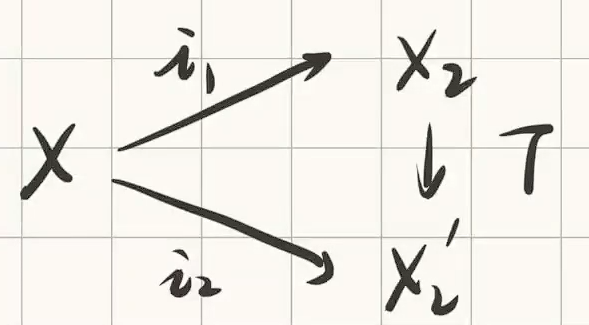
\includegraphics[width=0.4\linewidth]{figure/1.2.4-1}
					\caption{$X_2$ 在保距同构下的唯一性}
					\label{pic : 1.2.4-1} % 添加图像引用标签
				\end{figure}
			\end{enumerate}
		\end{proof}
		
		\vspace{1em}
		
		\begin{example}\label{ex 1.2.4}
			下面给出两个完备化空间的例子.
			\begin{enumerate}
				\item  $(P[a , b] , \rho_\infty) \rightarrow (C[a , b] , \rho_\infty)$, 即区间$[a , b]$ 上的多项式全体在度量$\rho_\infty$ 下的完备化空间为$[a , b]$ 上的连续函数全体. 其中
				\begin{align}
					\rho_\infty(x , y) = \max_{a \leq t \leq b}{\left| x(t) - y(t) \right|}
				\end{align}
				
				\item $(C[a , b] , \rho_1) \rightarrow (L^1[a , b] , \rho_1)$, 即区间$[a , b]$ 上的连续函数全体在度量$\rho_1$ 下的完备化空间为$[a , b]$ 上Lebesgue可积函数全体.
			\end{enumerate}
		\end{example}
	\end{thm}

\newpage

\section{Sequentially Compact}
\paragraph{引入}
	回顾在拓扑和数学分析中接触过的概念, \textbf{列紧性 (sequentially compact)}. 现将其限制于\textbf{度量空间}上给出定义.
	\begin{defn}\label{def 1.3.1}
		Suppose $(X , \rho)$ be a metric space, $A \subset X$. If $\forall \{ x_n \}_{n = 1}^{\infty} \subset A$, $\exists$ subsequence $\{ x_{n_k} \}_{k = 1}^{\infty} \subset \{ x_n \}_{n = 1}^{\infty}$ convergent in $X$, then we call $A$ \underline{\textcolor{blue}{\textbf{sequentially compact (列紧的)}}}.
		
		\vspace{2em}
		
		\begin{rmk}
			\begin{itemize}
				\item 将条件``\textbf{metric space $(X , \rho)$}"改为``\textbf{拓扑空间$X$}"即可得到拓扑中的一般性定义. 回顾一般拓扑空间中``\textbf{紧致}"、``\textbf{列紧}"、``\textbf{极限点紧}"的定义与性质, 有如下关系:
				
				\begin{figure}[thbp!]
					\centering
					
\includegraphics[width=0.5\linewidth]{figure/1.3-1}
					\caption{Relations among \textbf{compact}, \textbf{sequentially compact} and \textbf{limit point compact}}
					\label{pic : 1.3-1} % 添加图像引用标签
				\end{figure}
				
				\vspace{1em}
				
				\item If $\forall \{ x_n \}_{n = 1}^{\infty} \subset A$, $\exists$ subsequence $\{ x_{n_k} \}_{k = 1}^{\infty} \subset \{ x_n \}_{n = 1}^{\infty}$ convergent in $A$, then 称$A$ \underline{\textcolor{blue}{\textbf{自列紧}}}.
			\end{itemize}
		\end{rmk}
	\end{defn}

\vspace{5em}
\paragraph{例子}
	下面给出一个经典的\textbf{非列紧空间}的例子.
	\begin{example}\label{ex 1.3.1}
		Consider the set 
		\begin{align}
			l^1 = \left\{ \{ x_n \}_{n = 1}^{\infty} \mid \sum_{n = 1}^{\infty}{\left| x_n \right|} < \infty , \,\, x_n \in \R \right\}
		\end{align}
		$\forall \xi = \{ x_n \}_{n = 1}^{\infty} , \eta = \{ y_n \}_{n = 1}^{\infty} \in l^1$, define the metric $\rho_1$ on $l^1$:
		\begin{align}
			\rho_1 : l^1 \times l^1 &\longrightarrow \R_{\geq 0} \\
			(\xi , \eta) &\longmapsto \rho_1(\xi , \eta) = \sum_{n = 1}^{\infty}{\left| x_n - y_n \right|}
		\end{align}
		Let
		\begin{align}
			A &= \left\{ \{ \delta_{kj} \}_{j = 1}^{\infty} \right\}_{k = 1}^{\infty} \\
			&= \left\{ (1 , 0 , \cdots , 0 , \cdots) , (0 , 1 , \cdots , 0 , \cdots) , \cdots , (0 , 0 , \cdots , 1 , \cdots) , \cdots \right\}
			\subset l^1
		\end{align}
		则$A \subset l^1$ 中每两个元素之间的距离均为$2$, 无收敛子列, 故$(l^1 , \rho_1)$ 非列紧.
	\end{example}

\newpage

\paragraph{性质}
	对于\textbf{度量空间中的列紧集}, 容易得到其必为\textbf{完备度量空间}.
	\begin{proposition}\label{prop 1.3.1}
		\begin{center}
			列紧度量空间必完备.
		\end{center}
		
		\vspace*{4em}
		
		\begin{proof}
			Suppose $(X , \rho)$ be sequentially compact. Then for $\forall$ Cauchy sequence $\{ x_n \}_{n = 1}^{\infty} \subset X$, \\
			$\exists$ subsequence $\{ x_{n_k} \}_{k = 1}^{\infty}$ convergent $\,\, \Rightarrow \,\,$ Cauchy sequence $\{ x_n \}_{n = 1}^{\infty}$ convergent $\,\, \Rightarrow \,\,$ $(X , \rho)$ complete
		\end{proof}
	\end{proposition}

\vspace*{6em}

	为了更好地理解一般度量空间中的\textbf{列紧性}, 我们可以与欧氏空间$\R^n$ 中\textbf{有界}的概念联系.
	\vspace*{1em}
	\begin{center}
		\begin{tabular}{c|c}
			$\R^n$ &\text{度量空间} \\
			\hline
			\textbf{有界 ($bounded$)} &\textbf{列紧} \\
			\hline
			\textbf{有界闭} &\textbf{自列紧}
		\end{tabular}
	\end{center}

\newpage

\section{完全有界集}
\paragraph{$\epsilon$-网}
	在一般的度量空间中, 我们来引入一个比\textbf{有界集}更强的概念. 首先来给出\textbf{$\epsilon$-网}的定义.
	\begin{defn}\label{def 1.4.1}
		Suppose $(X , \rho)$ be a metric space, $N \subset M \subset X$ and $\epsilon > 0$. If for $\forall x \in M$, $\exists y \in N$, $\st$
		\begin{center}
			$\rho(x , y) < \epsilon$
		\end{center}
		则称$N$ 为$M$ 的一个\underline{\textcolor{blue}{\textbf{$\epsilon$-网}}}, 即$M \subset \underset{x \in N}{\bigcup}{B(x , \epsilon)}$. 进一步若$N$ 为有穷集 ($finite$), 则称$N$ 为$M$ 的一个\underline{\textcolor{blue}{\textbf{有穷$\epsilon$-网}}}.
	\end{defn}
	
	\vspace*{6em}
\paragraph{完全有界集}
	下面给出\textbf{完全有界集}的概念.
	\begin{defn}\label{def 1.4.2}
		Suppose $(X , \rho)$ be a metric space, $A \subset X$. If $\forall \epsilon > 0$, $A$ 存在有穷$\epsilon$-网, 则称$A$ 为\underline{\textcolor{blue}{\textbf{完全有界集}}}.
		
		\vspace*{2em}
		\begin{rmk}
			\textbf{完全有界集}的概念比\textbf{有界集}要更强, 即
			\begin{center}
				\textbf{完全有界集} $\,\, \Rightarrow \,\,$ \textbf{有界集} \hspace*{1em} , \hspace*{1em} \textbf{完全有界集} $\,\, \not\Leftarrow \,\,$ \textbf{有界集}
			\end{center}
			\vspace*{1em}
			\textbf{例\ref{ex 1.3.1}} 中集合$A = \left\{ \left\{ \delta_{kj} \right\}_{j = 1}^{\infty}  \right\}_{k = 1}^{\infty}$ 即为有界集但非\textbf{完全有界}.
		\end{rmk}
	\end{defn}

\vspace*{6em}
\paragraph{等价表述}
	下面我们将给出一般度量空间中\textbf{完全有界集的等价表述}, 便于我们判断和理解\textbf{完全有界集}的概念.
	
	\newpage
	\begin{thm}\label{thm 1.4.1}
		\textbf{完全有界集的等价表述}. \\
		Suppose $(X , \rho)$ be a metric space and $A \subset X$. Then
		\begin{center}
			$A$ 完全有界 $\,\, \Leftrightarrow \,\,$ $A$ 中任意点列存在$Cauchy$ 子列
		\end{center}
		
		\vspace*{2em}
		
		\begin{rmk}
			根据该定理我们容易得到, 在\textbf{一般的度量空间}中, \textbf{列紧} $\,\, \Rightarrow \,\,$ \textbf{完全有界}. 而在\textbf{完备度量空间}中, \textbf{完全有界} $\,\, \Leftrightarrow \,\,$ \textbf{列紧}. 特别地, 在欧氏空间$\R^n$ 中, \textbf{列紧}、\textbf{完全有界}、\textbf{有界}三者等价.
		\end{rmk}
		
		\vspace*{2em}
		
		\begin{proof}
			\begin{enumerate}
				\item[$\Rightarrow$]: 若$A$ 完全有界. $\forall \{ x_n \}_{n = 1}^{\infty} \subset A$, 下面证明$\{ x_n \}_{n = 1}^{\infty}$ 存在$Cauchy$ 子列: 
				
				\vspace*{1em}
				
				\begin{itemize}
					\item For $\epsilon = 1$, $\exists y_1 \in A$, $\st B(y_1 , 1)$ 中包含$\{ x_n \}_{n = 1}^{\infty}$ 无穷多项, 记为$\{ x_{n}^{(1)} \}_{n = 1}^{\infty} \subset \{ x_n \}_{n = 1}^{\infty}$.
					\begin{center}
						(否则若$\forall y \in A$, $B(y , 1)$ 均至多包含$\{ x_n \}_{n = 1}^{\infty}$ 中有穷个点, 则$A$ 无有穷$1$-网)
					\end{center}
				
					\vspace*{1em}
					
					\item For $\epsilon = \dfrac{1}{2}$, $\exists y_2 \in A$, $\st B(y_2 , \dfrac{1}{2})$ 中包含$\{ x_{n}^{(1)} \}_{n = 1}^{\infty}$ 无穷多项, 记为$\{ x_{n}^{(2)} \}_{n = 1}^{\infty} \subset \{ x_{n}^{(1)} \}_{n = 1}^{\infty}$.
					\begin{center}
						$\cdots$
					\end{center}
					
					\item For $\epsilon = \dfrac{1}{k}$, $\exists y_k \in A$, $\st B(y_k , \dfrac{1}{k})$ 中包含$\{ x_{n}^{(k - 1)} \}_{n = 1}^{\infty}$ 中无穷多项, 记为$\{ x_{n}^{(k)} \}_{n = 1}^{\infty} \subset \{ x_{n}^{(k - 1)} \}_{n = 1}^{\infty}$.
				\end{itemize}
				
				\vspace*{1em}
				
				从而我们得到了$\{ x_n \}_{n = 1}^{\infty}$ 的一列子列: $\{ x_{n}^{(1)} \}_{n = 1}^{\infty} , \{ x_{n}^{(2)} \}_{n = 1}^{\infty} , \cdots , \{ x_{n}^{(k)} \}_{n = 1}^{\infty} , \cdots$ \\
				取出第$k$ 个子列$\{ x_{n}^{(k)} \}_{n = 1}^{\infty}$ 的第$k$ 项$x_{k}^{(k)}$, 得到子列$\{ x_{n}^{(n)} \}_{n = 1}^{\infty}$\footnote{这种从一列序列中各取出一个元素构成新序列, 再(一致)收敛的方法称为\textbf{对角线法则}, 在\textbf{实分析 ($Real \,\, Analysis$)}中证明\textbf{任一可测函数可由简单函数列逼近}时曾使用, 详情可见$Real \,\, Analysis$ 笔记\textbf{定理 2.2.1}.}. \\
				下面证明:$\{ x_{n}^{(n)} \}_{n = 1}^{\infty} \subset \{ x_n \}_{n = 1}^{\infty}$ 为$Cauchy$ 列.\\
				Since
				\begin{align}
					\rho(x_{n + p}^{(n + p)} , x_{n}^{(n)}) 
					\leq \rho(x_{n + p}^{(n + p)} , y_n) + \rho(y_n , x_{n}^{(n)}) 
					\leq \frac{2}{n} , \,\, \forall n , p \in \N
				\end{align}
				Therefore, $\{ x_{n}^{(n)} \}_{n = 1}^{\infty} \subset \{ x_n \}_{n = 1}^{\infty}$ is a Cauchy sequence in $A$.
				
				\newpage
				
				\item[$\Leftarrow$]: 反证法. Assume $A$ 非完全有界, 即$\exists \epsilon_0 > 0$, $\st A$ 无有穷$\epsilon_0$-网.  
				
				\vspace*{1em}
				
				\begin{itemize}
					\item $\forall x_1 \in A$, $\exists x_2 \in A \backslash B(x_1 , \epsilon_0)$ (Otherwise $A \subset B(x_1 , \epsilon_0)$, $A$ 存在有穷$\epsilon_0$-网)
					
					\item Similarly, $\exists x_3 \in A \backslash \left( B(x_1 , \epsilon_0) \cup B(x_2 , \epsilon_0) \right)$
					
					\begin{center}
						$\cdots$
					\end{center}
				
					\item $\exists x_k \in A \backslash \left( \bigcup_{i = 1}^{k - 1}{B(x_i , \epsilon_0)} \right)$
				\end{itemize}
			
				\vspace*{1em}
				
				从而得到$A$ 中的一列点$\{ x_n \}_{n = 1}^{\infty} \subset A$, 其中
				\[ \rho(x_i , x_j) > \epsilon_0 > 0 , \,\, \forall i \neq j \]
				于是$\{ x_n \}_{n = 1}^{\infty} \subset A$ 无Cauchy子列, 矛盾.
			\end{enumerate}
		\end{proof}
	\end{thm}

\newpage

\section{可分度量空间}
	作为一类特殊的\textbf{拓扑空间}, 下面我们来讨论一些常见的\textbf{度量空间}的\textbf{可分性}. 首先回顾一下\textbf{可分}的定义.
	\begin{defn}\label{def 1.5.1}
		Suppose $(X , \tau)$ be a Topological space. If $(X , \tau)$ 存在\textbf{可数稠密子集}, then $(X , \tau)$ is called \underline{\textcolor{blue}{\textbf{separable (可分的)}}}.
	\end{defn}
	
	\vspace*{6em}
	
	根据\textbf{可分空间}的定义, 不难得到上节所介绍的\textbf{完全有界空间可分}.
	
	\begin{proposition}\label{prop 1.5.1}
		完全有界空间为可分度量空间.
		
		\vspace*{4em}
		
		\begin{proof}
			Suppose $(X , \rho)$ is totally bounded. Then for $\forall k \in \N$, $\exists n_k \in \N ,  y_{1} , \cdots , y_{n_k} \in X$, $\st$
			\begin{align}
				X \subset \bigcup_{i = 1}^{n_k}{B(y_{i}^k , \frac{1}{k})}
			\end{align}
			Let
			\begin{align}
				A = \bigcup_{k = 1}^{\infty} \bigcup_{i = 1}^{n_k}{\{ y_{i}^k \}} \subset X \,\, countable
			\end{align}
			Then for $\forall x \in X$, $\exists 1 \leq l_k \leq n_k , y_{l_k}^{k} \in A$, $\st$
			\[ \rho(x , y_{l_k}^k) < \dfrac{1}{k} , \,\, \forall k \in \N \]
			Thus $\{ y_{l_k}^k \}_{k = 1}^{\infty} \subset A$ convergent to $x \in X$, i.e. $y_{l_k}^k \overset{\rho}{\to} x$ as $k \to \infty$. \\
			Therefore, by \textbf{Lemma \ref{lemma A.1.1}}, $A \subset X$ is dense in $X$. $X$ is separable.
		\end{proof}
	\end{proposition}
	
	\vspace*{6em}
	
	下面来讨论一些常见的\textbf{度量空间}的\textbf{可分性}.
	
	\newpage
	
	\begin{example}\label{ex 1.5.1}
		\textbf{[可分空间]}. 
		\begin{itemize}
			\item $(C[a , b] , \rho_{\infty})$ 可分. 
			
			\begin{itemize}
				\item 
				\begin{proof}
					有理系数多项式 $\,\, \overset{\text{一致逼近}}{\Longrightarrow} \,\,$ 多项式 $\,\, \overset{\text{一致逼近}}{\Longrightarrow} \,\,$ 连续函数
				\end{proof}
			\end{itemize}
			
			\vspace*{0.75em}
			
			\item $(l^p , \rho_p)$ 可分.
			
			\begin{itemize}
				\item 
				\begin{proof}
					此处$(l^p , \rho_p)$ 定义与\textbf{例 \ref{ex 1.3.1}} 中一致, 即
					\begin{align}
						l^p &= \left\{ \{ x_n \}_{n = 1}^{\infty} \mid \sum_{n = 1}^{\infty}{\left| x_n \right|^p} < \infty , \,\, x_n \in \R \right\} \\
						\rho_p : l^p \times l^p &\longrightarrow \R_{\geq 0} \\
						(\{ x_n \}_{n = 1}^{\infty} , \{ y_n \}_{n = 1}^{\infty}) &\longmapsto \rho_p(\{ x_n \}_{n = 1}^{\infty} , \{ y_n \}_{n = 1}^{\infty}) = \sum_{n = 1}^{\infty}{\left| x_n - y_n \right|^p}
					\end{align}
					下面来构造$(l^p , \rho_p)$ 的可数稠密子集:
					
					\begin{itemize}
						\item Let
						\begin{align}
							A_1 &= \left\{ \{ x_n \}_{n = 1}^{\infty} \mid x_1 \in \Q , \,\, x_n = 0 , \,\, \forall n > 1 \right\} \subset l^p \\
							A_2 &= \left\{ \{ x_n \}_{n = 1}^{\infty} \mid x_1 , x_2 \in \Q , \,\, x_n = 0 , \,\, \forall n > 2 \right\} \subset l^p \\
							\cdots & \\
							A_k &= \left\{ \{ x_n \}_{n = 1}^{\infty} \mid x_1 , \cdots , x_k \in \Q , \,\, x_n = 0 , \,\, \forall n > k \right\} \subset l^p \\
							A &= \bigcup_{k = 1}^{\infty}{A_k} \subset l^p
						\end{align}
						
						\item $A \subset l^p$ 即为$(l^p , \rho_p)$ 的可数稠密子集: \\
						$\forall \{ x_n \}_{n = 1}^{\infty} \in l^p$. Since 
						\[ \sum_{n = 1}^{\infty}{\left| x_n \right|^p} < \infty \]
						Then for $\forall \epsilon > 0$, $\exists N \in \N$, $\st$
						\[ \sum_{n = N + 1}^{\infty}{\left| x_n \right|^p} < \dfrac{\epsilon}{2} \]
						Thus $\exists \{ y_n \}_{n = 1}^{\infty} \in A_N \subset A$, $y_n = 0$, $\forall n > N$ and
						\[ \left| y_n - x_n \right|^p < \dfrac{\epsilon}{2N} , \,\, \forall 1 \leq n \leq N \]
						Therefore
						\[ \rho_p(\{ x_n \}_{n = 1}^{\infty} , \{ y_n \}_{n = 1}^{\infty}) 
						= \sum_{n = 1}^{\infty}{\left| x_n - y_n \right|^p} 
						< \epsilon \]
						$A \subset l^p$ is dense in $l^p$ while it's also countable.
					\end{itemize}
				\end{proof}
			\end{itemize}
			
			\newpage
			
			\item $L^{p}[a , b]$ 可分. 
			\begin{proof}
				Review the conclusions in $Real \,\, Analysis$. $\forall f \in L^{p}[a , b]$, then $f$ is measurable.\\
				Since \textbf{任一可测函数可由简单函数列逼近 ($Real \,\, Analysis$ 笔记Thm 2.2.1)} \\
				又根据\textbf{Lusin定理 ($Real \,\, Analysis$ 笔记Thm 3.8.2)}, 可得:
				\begin{center}
					连续函数 $\,\, \Rightarrow \,\,$ 简单函数 $\,\, \Rightarrow \,\,$ $f \in L^p$
				\end{center}
			\end{proof}
			
			\vspace*{2em}
			
			\item $L^{\infty}[a , b]$ 不可分.
			\begin{proof}
				Let
				\begin{align}
					E = \left\{ f \in L^{\infty}[a , b] \,\, \Big| \,\, f(x) = 
					\begin{cases}
						0 , x \in [a , r] \\
						1 , x \in (r , b]
					\end{cases} , \,\, \forall r \in (a , b) \right\}
				\end{align}
				Then $E \subset L^{\infty}[a , b]$ is uncountable, and
				\[ \rho_{\infty}(f , g) = 1 > 0 , \,\, \forall f , g \in E \]
				下面用反证法证明$L^{\infty}[a , b]$ 不可分. Assume $L^{\infty}[a , b]$ is separable. \\
				Then $\exists$ countable $\{ f_n \}_{n = 1}^{\infty} \subset L^{\infty}[a , b]$, $\st$
				\[ \overline{\{ f_n \}_{n = 1}^{\infty}} = L^{\infty}[a , b] \]
				即$L^{\infty}[a , b]$ 中点均可由$\{ f_n \}_{n = 1}^{\infty}$ 中的某些点逼近, 从而
				\[ \bigcup_{n = 1}^{\infty}{B(f_n , \dfrac{1}{3})} = L^{\infty}[a , b] \supset E \]
				于是$\exists N \in \N$, $\st$
				\begin{center}
					$B(f_N , \dfrac{1}{3})$ 中包含$E$ 中至少2个点 (事实上可严格地说包含$E$ 中不可数个点)
				\end{center}
				而$\rho_{\infty}(f , g) = 1 > 0 , \,\, \forall f , g \in E$, 这与$f , g \in B(f_N , \dfrac{1}{3})$ 矛盾. \\
				综上, $L^{\infty}[a , b]$ 不可分.
			\end{proof}
		
			\newpage
			
			\item $l^{\infty}$ 不可分.
			\begin{proof}
				Similarly. Let
				\begin{align}
					E = \left\{ \{ x_n \}_{n = 1}^{\infty} \in l^{\infty} \mid x_n = 0 \,\, or \,\, 1 , \,\, \forall n \in \N \right\} \subset l^{\infty}
				\end{align}
				Then $E \subset l^{\infty}$ is uncountable ($E$ 与二进制数一一对应, 而二进制数与实数$\R$ 一一对应), and
				\[ \rho_{\infty}(\{ x_n \}_{n = 1}^{\infty} , \{ y_n \}_{n = 1}^{\infty}) = 1 > 0 , \,\, \forall \{ x_n \}_{n = 1}^{\infty} , \{ y_n \}_{n = 1}^{\infty} \in E \]
				后续步骤与上述$L^{\infty}[a , b]$ 不可分证明过程一致.
			\end{proof}
		\end{itemize}
	\end{example}

\newpage

\section{Compact}
	首先来回顾一下\textbf{拓扑学}中关于\textbf{紧致}的定义, 在度量空间中也是一脉相承的.
	\begin{defn}\label{def 1.6.1}
		Suppose $(X , \tau)$ be a topological space. If $X$ 的任意开覆盖都有有限子覆盖, 则称$X$ 为\underline{\textcolor{blue}{\textbf{紧致的 (compact)}}}.
		
		\vspace{2em}
		
		\begin{rmk}
			事实上我们运用的更多的为\textbf{一般拓扑 / 度量空间}的\textbf{紧致子集}的概念, 其定义如下:
			\begin{center}
				Suppose $A \subset (X , \tau)$. If $A$ 的任意开覆盖都有有限子覆盖 (在子空间拓扑意义下为紧集), 则\\
				称$A$ 为\underline{\textcolor{blue}{\textbf{紧(子)集}}}.
			\end{center}
		\end{rmk}
	\end{defn}

\vspace{2em}
\subsection{度量空间紧集的性质}	
	下面我们给出度量空间中紧集的4条性质(事实上大部分对一般的Hausdorff空间成立).
	
	\begin{proposition}\label{prop 1.6.1}
		\textbf{[紧$\Rightarrow$ 闭, Hausdorff]}. 
		\begin{center}
			若$A \subset (X , \rho)$ 紧致, 则$A$ 为闭集.
		\end{center}
		
		\vspace{2em}
		
		\begin{rmk}
			该结论对于一般拓扑空间不成立, 但对于\textbf{Hausdorff空间}成立, 故自然\textbf{度量空间}成立.
		\end{rmk}
	
		\vspace{2em}
		
		\begin{proof}
			下面对一般情形进行证明, 即$(X , \tau)$ 为Hausdorff空间, 证明:$A^c$ open. \\
			Fix $x \in A^c$. Since $X$ is Hausdorff, then for $\forall y \in A$, $\exists x \in V_{y}^x , y \in U_{y}^x$, $\st$
			\[ U_{y}^x \cap V_{y}^x = \varnothing , \,\, U_{y}^{x} , V_{y}^x \underset{open}{\subset} X \]
			Then we have
			\[ A \subset \bigcup_{y \in A} U_{y}^x \]
			Since $A$ is compact, there exists $U_{y_1}^x , \cdots , U_{y_n}^x \in \{ U_{y}^x \}_{y \in A}$, $\st$
			\[ A \subset \bigcup_{i = 1}^{n} U_{y_i}^x \]
			Let
			\[ V^x = \bigcap_{i = 1}^{n} V_{y_i}^x \underset{open}{\subset} X \]
			Then $x \in V^x$ and $V^x \cap \bigcup_{i = 1}^{n} U_{y_i}^x = \varnothing$, so $V^x \cap A = \varnothing , V^x \subset A^c$. Therefore, $A^c$ is open.
		\end{proof}
	\end{proposition}

	\newpage
	
	\begin{proposition}\label{prop 1.6.2}
		\textbf{[紧集的闭子集必为紧集, 一般拓扑空间]}. 
		\begin{center}
			若$A \subset (X , \rho)$ 紧致, $K \subset A$ 为闭集, 则$K$ 紧致.
		\end{center}
		
		\begin{rmk}
			该结论对于\textbf{一般的拓扑空间}均成立. 
		\end{rmk}
	
		\vspace{1em}
		
		\begin{proof}
			下面对一般情形进行证明, 且下述证明过程均以子空间$(A , \tau_A)$ 作为全空间. \\
			$\forall \{ U_i \}_{i \in I}$, $U_i \underset{open}{\subset} X$, $\forall i \in I$, $\st$
			\[ K \subset \bigcup_{i \in I}{U_i} \]
			Since $K \subset A$ closed, then $K^c \subset A$ open. Thus
			\[ A = K^c \cup K = K^c \cup \bigcup_{i \in I} U_i \]
			Since $A$ is compact, then $\exists i_1 , \cdot , i_n \in I$, $\st$
			\[ A = K^c \cup \bigcup_{k = 1}^{n} U_{i_k} \]
			Therefore $K \subset \bigcup_{k = 1}^{n} U_{i_k}$. $K \subset A$ is compact.
		\end{proof}
	\end{proposition}
	
	\vspace{8em}
	
	根据\textbf{命题 \ref{prop 1.6.2}}, 我们可得到另一条直接推论.
	\begin{corollary}\label{cor 1.6.1}
		\textbf{[Hausdorff]}. 
		\begin{center}
			\textbf{紧集和闭集的交为紧集}.
		\end{center}
		
		\vspace{1em}
		
		\begin{proof}
			紧集与闭集相交 $\,\, \Rightarrow \,\,$ 交集为原紧集的闭子集 $\,\, \Rightarrow \,\,$ 根据\textbf{命题 \ref{prop 1.6.2}}, 该交集为紧集
		\end{proof}
	\end{corollary}

	\newpage
	
	\begin{proposition}\label{prop 1.6.3}
		\textbf{[Hausdorff]}. \\
		$\{ K_\alpha \subset X \}_{\alpha \in \Lambda}$ 为一个紧子集族, 满足任意有限交非空, 则
		\begin{align}
			\bigcap_{\alpha \in \Lambda} K_\alpha \neq \varnothing
		\end{align}
		
		\vspace{1em}
		
		\begin{proof}
			反证法. Assume $\underset{\alpha \in \Lambda}{\bigcap} K_\alpha = \varnothing$. Then for $\forall \alpha_0 \in \Lambda$,
			\[ K_{\alpha_0} \cap \bigcap_{\substack{\alpha \in \Lambda \\ \alpha \neq \alpha_0}} K_{\alpha} = \varnothing 
			\hspace*{2em} , \hspace*{2em} 
			K_{\alpha_0} \subset \bigcup_{\substack{\alpha \in \Lambda \\ \alpha \neq \alpha_0}} K_{\alpha}^c \]
			Since $X$ is Hausdorff, $K_\alpha \subset X$ is compact, then $K_\alpha$ is closed, $\forall \alpha \in \Lambda$. Thus \\
			$\{ K_{\alpha}^c \mid \alpha \neq \alpha_0 \}_{\alpha \in \Lambda}$ is an open covering of $K_{\alpha_0}$. Since $K_{\alpha_0} \subset X$ is compact, then $\exists \alpha_1 , \cdots , \alpha_n \in \Lambda$, $\st$
			\[ K_{\alpha_0} \subset \bigcup_{i = 1}^{n} K_{\alpha_i}^c \]
			Therefore, 
			\[ \bigcap_{i = 0}^{n} K_{\alpha_i} = \varnothing \]
			which is a contradiction to “任意有限交非空”.
		\end{proof}
	\end{proposition}
	
	\vspace{4em}
	
	\begin{proposition}\label{prop 1.6.4}
		\textbf{[Hausdorff]}. \\
		$A \subset (X , \rho)$ 为闭集. 若对于$A$ 中任意闭子集族$\{ F_\alpha \}_{\alpha \in \Lambda}$, 如果满足任意有限交非空, 便有$\underset{\alpha \in \Lambda}{\bigcap} F_\alpha \neq \varnothing$, 则$A$ 为紧集.
		
		\vspace{2em}
		
		\begin{proof}
			$\forall \{ U_i \}_{i \in I}$, $U_i \underset{open}{\subset} X$, $\forall i \in I$, $\st$
			\[ A \subset \bigcup_{i \in I} U_i \]
			Then $\{ U_{i}^c \cap A \}_{i \in I}$ 为$A$ 的闭子集族. Since 
			\[ \bigcap_{i \in I} U_{i}^c \cap A = \varnothing \]
			Then 根据条件, $\{ U_{i}^c \cap A \}_{i \in I}$ 存在有限交为空集, 即$\exists i_1 , \cdots , i_n \in I$, $\st$
			\[ \bigcap_{k = 1}^{n} U_{i}^c \cap A = A \cap \left( \bigcup_{k = 1}^{n} U_{i_k} \right)^c = \varnothing \]
			Thus
			\[ A \subset \bigcup_{k = 1}^{n} U_{i_k} \]
			Therefore, $A \subset X$ is compact.
		\end{proof}
	\end{proposition}

\newpage

\subsection{度量空间紧致的等价刻画}
	下面我们将说明, 在\textbf{度量空间}中, \textbf{紧致性}与\textbf{自列紧性}等价.
	
	\begin{thm}\label{thm 1.6.2}
		\textbf{[紧致$\Leftrightarrow$ 自列紧, 度量空间]}. \\
		在度量空间$(X , \rho)$ 中, 
		\begin{center}
			\textbf{$A \subset X$ 紧致} $\,\, \Leftrightarrow \,\,$ \textbf{自列紧}
		\end{center}
	
		\vspace{4em}
		
		\begin{proof}
			\begin{enumerate}
				\item[$\Rightarrow$]: 只需考虑$A$ 中无穷点集的情形. $\forall$ 无穷点集$\{ x_n \}_{n = 1}^{\infty} \subset A$, 不妨设$x_n$ 互异. \\
				反证法. Assume $\{ x_n \}_{n = 1}^{\infty} \subset A$ 在$A$ 中无聚点, 则$\forall x \in A$, $\exists U_x \underset{open}{\subset} X$, $\st$
				\[ U_x \cap \{ x_n \}_{n = 1}^{\infty} \subset \{ x \} \hspace{2em} \left( = \varnothing \,\, \text{or} \,\, \{ x \} \right) \]
				Since $A \subset \bigcup_{x \in A} U_x$, $A$ is compact, then $\exists y_1 , \cdots , y_n \in A$, $\st$
				\[ \{ x_n \}_{n = 1}^{\infty} \subset A \subset \bigcup_{i = 1}^{n} U_{y_i} \]
				从而$\{ U_{y_i} \}_{i = 1}^{n}$ 中至少有一项中包含$\{ x_n \}_{n = 1}^{\infty}$ 中无穷多项, 这与$U_x \cap \{ x_n \}_{n = 1}^{\infty} \subset \{ x \}$ 矛盾. \\
				综上, $A \subset X$ 紧致 $\,\, \Rightarrow \,\,$ 自列紧.
				
				\vspace{6em}
				
				\item[$\Leftarrow$]: 反证法. 假设$\exists A$ 的一个开覆盖$\{ U_\alpha \}_{\alpha \in \Lambda}$ 不存在有限子覆盖. \\
				Since $A$ 自列紧 $\,\, \Rightarrow \,\,$ 列紧 $\,\, \Rightarrow \,\,$ 完全有界 (\textbf{Thm \ref{thm 1.4.1}}), then for $\forall$ fixed $n \in \N$, \\
				$A$ 存在有穷$\dfrac{1}{n}$-网, i.e. $\exists M_n$ finite, $\st$
				\[ A \subset \bigcup_{x \in M_n} B(x , \frac{1}{n}) \]
				Then for the fixed $n$, $\exists x_n \in M_n$, $\st B(x_n , \dfrac{1}{n})$ 不能被$\{ U_\alpha \}_{\alpha \in \Lambda}$ 有限覆盖.
				\begin{center}
					(否则若$\forall x \in M_n$, $B(x , \dfrac{1}{n})$ 均可被$\{ U_\alpha \}_{\alpha \in \Lambda}$ 有限覆盖, 则$A \subset \bigcup_{x \in M_n} B(x , \dfrac{1}{n})$ 可被$\{ U_\alpha \}_{\alpha \in \Lambda}$ 有限覆盖. 矛盾)
				\end{center}
				Then we get a sequence $\{ x_n \}_{n = 1}^{\infty} \subset A$ in $A$. \\
				Since $A$ 自列紧, then $\exists$ subsequence $\{ x_{n_k} \}_{k = 1}^{\infty} \subset \{ x_n \}_{n = 1}^{\infty}$, $\st$
				\[ x_{n_k} \to x_0 \in A \,\, as \,\, k \to \infty \]
				Since $\{ U_\alpha \}_{\alpha \in \Lambda}$ covers $A$, then $\exists \alpha_0 \in \Lambda$, $\st x_0 \in U_{\alpha_0}$. \\
				Since $U_{\alpha_0}$ is open, then $\exists \epsilon > 0$, $\st B(x_0 , \epsilon) \subset U_{\alpha_0}$. \\
				However, since $x_{n_k} \to x_0$, for $\epsilon > 0$, $\exists k_0 \in \N$, $\st$
				\[ \rho(x_{n_{k_0}} , x_0) < \frac{\epsilon}{3} \,\, \text{and} \,\, \frac{1}{n_{k_0}} < \frac{\epsilon}{3} \]
				Then $B(x_{n_{k_0}} , \dfrac{1}{n_{k_0}}) \subset U_{\alpha_0}$, 于是$B(x_{n_{k_0}} , \dfrac{1}{n_{k_0}})$ 被$\{ U_\alpha \}_{\alpha \in \Lambda}$ 有限覆盖, 矛盾. \\
				综上, $A$ 自列紧 $\,\, \Rightarrow \,\,$ compact.
			\end{enumerate}
		\end{proof}
	\end{thm}

\newpage

\section{一致有界, 等度连续}
	为了给出上\textbf{$C[a , b]$ (列)紧集的刻画}, 即下节介绍的\textbf{Arzel\`{a}-Ascoli定理}, 本节来给出一些前置概念.
\subsection{紧致度量空间上的连续函数全体}
	首先来给出\textbf{紧致度量空间$X$} 上的连续函数全体$C(X)$, 并赋予相应的\textbf{度量(无穷范数)}, 使其称为\textbf{完备度量空间}. 
	\begin{defn}\label{def 1.7.1}
		设$(X , \rho)$ 为紧致度量空间, 其上的\underline{\textcolor{blue}{\textbf{连续函数全体$C(X)$}}} 被定义为:
		\begin{align}
			C(X) \coloneqq \{ f : X \longrightarrow \mathbb{K} \mid f \,\, \text{continuous} \} , \,\, \mathbb{K} \in \{ \C , \R \}
		\end{align}
		赋予$C(X)$ 上度量$d$, 定义为:
		\begin{align}
			d : C(X) \times C(X) &\longrightarrow \R_{\geq 0} \\
			(f , g) &\longmapsto \max_{x \in X} \left| f(x) - g(x) \right|
		\end{align}
		
		\vspace{2em}
		
		\begin{rmk}
			\begin{itemize}
				\item 不难证明上述定义的度量$d$ 满足\textbf{度量的三大公理 (Def \ref{def 1.1.2})}. 关于其定义是否\textbf{良好(Well-defined)}的问题, 只需说明对于$\forall f , g \in C(X)$, $d(f , g)$ 的存在性:
				
				\vspace{3em}
				
				\begin{itemize}
					\item 
					\begin{proof}
						不难证明$C(X)$ 为线性空间, 于是对于$\forall f , g \in C(X)$, $f - g \in C(X)$. \\
						根据\textbf{绝对值不等式}, 容易得到绝对值保持$C(X)$ 中函数的连续性. 
						\begin{center}
							($\left| \left| \varphi(x) \right| - \left| \varphi(y) \right| \right| \leq \left| \varphi(x) - \varphi(y) \right| , \,\, \forall \varphi \in C(X) , x , y \in X$)
						\end{center}
						因此$\left| f - g \right| \in C(X)$, 即连续. \\
						Since $X$ is compact, then $\left| f - g \right| (X) \subset \R_{\geq 0}$ compact, 可取到最大值. 故$d(f , g)$ 存在.
					\end{proof}
				\end{itemize}
				
				\vspace{4em}
				
				\item 事实上, 上述定义的度量空间$(C(X) , d)$ 是\textbf{完备的}, 这在下面的\textbf{命题 \ref{prop 1.7.1}} 中得以证明.
			\end{itemize}
		\end{rmk}
	\end{defn}

	\newpage
	
	下面的命题证明了, \textbf{定义 \ref{def 1.7.1}} 中定义的度量空间$(C(X) , d)$ 是完备的.
	
	\begin{proposition}\label{prop 1.7.1}
		\textbf{$(C(X) , d)$ 为完备度量空间}.
		
		\vspace{2em}
		
		\begin{proof}
			$\forall$ Cauchy sequence $\{ f_n \}_{n = 1}^{\infty} \subset C(X)$, i.e. $\forall \epsilon > 0$, $\exists N_\epsilon \in \N$, $\st$
			\[ d(f_m , f_n) = \max_{x \in X} \left| f_{m}(x) - f_{n}(x) \right| < \epsilon , \,\, \forall m , n \geq N_\epsilon \]
			下面分两步进行证明:
			\begin{enumerate}
				\item $\exists f : X \longrightarrow \mathbb{K}$, $\st f(x) = \underset{n \to \infty}{\lim} f_{n}(x) , \,\, \forall x \in X$:\\
				Since $\underset{x \in X}{\max} \left| f_{m}(x) - f_{n}(x) \right| < \epsilon , \,\, \forall m , n \geq N_\epsilon$, then 
				\[ \left| f_{m}(x) - f_{n}(x) \right| < \epsilon , \,\, \forall x \in X , \,\, \forall m , n \geq N_\epsilon \]
				Thus $\forall x \in X$, fix $x$. $\{ f_{n}(x) \}_{n = 1}^{\infty} \subset \mathbb{K}$ is a Cauchy sequence in $\mathbb{K}$. \\
				Since both $\C$ and $\R$ are complete, then $\{ f_{n}(x) \}_{n = 1}^{\infty}$ converges, $\forall x \in X$. Let
				\begin{align}
					f : X &\longrightarrow \mathbb{K} \\
					x &\longmapsto \lim_{n \to \infty} f_{n}(x)
				\end{align}
				Then $f$ is a mapping from $X$ to $\mathbb{K}$ with $f(x) = \underset{n \to \infty}{\lim} f_{n}(x) , \,\, \forall x \in X$.
				
				\vspace{4em}
				
				\item $f \in C(X)$, i.e. $f : X \longrightarrow \mathbb{K}$ continuous:\\
				Since 
				\[ \left| f_{m}(x) - f_{n}(x) \right| < \epsilon , \,\, \forall x \in X , \,\, \forall m , n \geq N_\epsilon \]
				Then letting $m \to \infty$, we get $f_n \Rightarrow f$, i.e.
				\[ \left| f(x) - f_{n}(x) \right| < \epsilon , \,\, \forall x \in X , \,\, \forall n \geq N_\epsilon \]
				For $f_{N_\epsilon} \in C(X)$, fix $\epsilon > 0$. Since $f_{N_\epsilon}$ continuous, $\exists \delta > 0$, $\st$
				\[ \left| f_{N_\epsilon}(x) - f_{N_\epsilon}(y) \right| < \epsilon , \,\, \forall \rho(x , y) < \delta \]
				Then for $\epsilon > 0$, $\exists \delta > 0 , N_\epsilon \in \N$, $\st$
				\begin{align}
					\left| f(x) - f(y) \right| 
					&\leq \left| f(x) - f_{N_{\epsilon}}(x) \right| + \left| f_{N_\epsilon}(x) - f_{N_\epsilon}(y) \right| + \left| f_{N_\epsilon}(y) - f(y) \right| \\
					&< 3\epsilon , \,\, \forall \rho(x , y) < \delta
				\end{align}
				Therefore, $f : X \longrightarrow \mathbb{K}$ is continuous, $f \in C(X)$. In short, $(C(X) , d)$ is complete.
			\end{enumerate}
		\end{proof}
	\end{proposition}

\newpage

\subsection{一致有界, 等度连续}
	下面我们来给出\textbf{一致有界}与\textbf{等度连续}的概念, 实际上为数学分析中\textbf{一致有界}与\textbf{一致连续}在更高维度上的一致性的推广, 即同时对函数和自变量都一致.
	
	\vspace{2em}
	
	\begin{defn}\label{def 1.7.2}
		\textbf{[一致有界]}. \\
		设$(X , \rho)$ 为紧致度量空间, $A \subset (C(X) , d)$. 若
		\[ \sup_{\substack{x \in X \\ \varphi \in A}} \left| \varphi(x) \right| < \infty \]
		则称\underline{\textcolor{blue}{\textbf{$A$ 一致有界}}}.
	\end{defn}

	\vspace{10em}
	
	\begin{defn}\label{def 1.7.3}
		\textbf{[等度连续]}. \\
		设$(X , \rho)$ 为紧致度量空间, $A \subset (C(X) , d)$. 若$\forall \epsilon > 0$, $\exists \delta > 0$, $\st$
		\[ \left| \varphi(x) - \varphi(y) \right| < \epsilon , \,\, \forall \rho(x , y) < \delta , \,\, \forall \varphi \in A \]
		则称\underline{\textcolor{blue}{\textbf{$A$ 等度连续}}}.
		
		\vspace{2em}
		
		\begin{rmk}
			相当于在数学分析\textbf{函数一致连续}的概念上增加了对$A$ 中所有函数的一致性.
		\end{rmk}
	\end{defn}

\newpage

\section{Arzel\`{a}-Ascoli定理}
	接下来我们将介绍\textbf{Arezel\`{a}-Ascoli定理}, 它给出了\textbf{紧致度量空间$X$ 上连续函数全体$(C(X) , d)$ 的(列)紧子集的等价刻画}.
	
	\begin{thm}\label{thm 1.8.1}
		\textbf{[Arezel\`{a}-Ascoli]}. \\
		设$(X , \rho)$ 为紧致度量空间, $A \subset C(X)$, 则:
		\begin{center}
			$A$ 列紧 $\,\, \Leftrightarrow \,\, A$ 一致有界且等度连续
		\end{center}
		
		\vspace{4em}
		
		\begin{proof}
			\begin{enumerate}
				\item[$\Rightarrow$]: 下面分两点分别证明一致有界和等度连续.
				\begin{itemize}
					\item $A$ 一致有界:Since $A$ 列紧 $\,\, \Rightarrow \,\,$ 完全有界, then for $\epsilon = 1$, $\exists \varphi_1 , \cdots , \varphi_n \in A$, $\st$
					\[ A \subset \bigcup_{i = 1}^{n} B(\varphi_i , 1) \]
					$\forall \varphi \in A$, WTS: $\exists M > 0$, $\st \left| \varphi(x) \right| \leq M , \,\, \forall x \in X$. \\
					$\exists 1 \leq i_0 \leq n$, $\st$
					\[ \varphi \in B(\varphi_{i_0} , 1) \]
					Then
					\[ d(\varphi , \varphi_{i_0}) = \max_{x \in X} \left| \varphi(x) - \varphi_{i_0}(x) \right| < 1 \]
					Thus
					\[ \left| \varphi(x) - \varphi_{i_0}(x) \right| < 1 , \,\, \forall x \in X \]
					Fix $1 \leq i \leq n$. For $\varphi_i \in A \subset C(X)$. \\
					Since $X$ is compact, $\varphi_i$ continuous, then $\varphi_{i}(X) \subset \mathbb{K}$ bounded, i.e. $\exists 0 < k_i < \infty$, $\st$
					\[ \left| \varphi_{i}(x) \right| \leq k_i , \,\, \forall x \in X \]
					Let $k = \underset{1 \leq i \leq n}{\max}{\{ k_i \}}$, then
					\begin{align}
						\left| \varphi(x) \right| 
						&\leq \left| \varphi(x) - \varphi_{i_0}(x) \right| + \left| \varphi_{i_0}(x) \right| \\
						&\leq 1 + k , \,\, \forall x \in X , \,\, \forall \varphi \in A
					\end{align}
					Therefore, $A \subset C(X)$ 一致有界.
					
					\newpage
					
					\item $A$ 等度连续:Since $A$ 列紧 $\,\, \Rightarrow \,\,$ 完全有界, then for $\forall \epsilon > 0$, $A$ 存在有穷$\epsilon$-网, i.e. \\
					$\exists \varphi_{1}^\epsilon , \cdots , \varphi_{i_\epsilon}^\epsilon \in A$, $\st$
					\[ A \subset \bigcup_{i = 1}^{i_\epsilon} B(\varphi_{i}^\epsilon , \epsilon) \]
					Since $\varphi_i \in C(X)$ continuous, $\forall 1 \leq i \leq i_\epsilon$, then for $\epsilon > 0$, $\exists \delta_{1}^\epsilon , \cdots , \delta_{i_\epsilon}^\epsilon > 0$, $\st$
					\[ \left| \varphi_{k}^\epsilon(x) - \varphi_{k}^\epsilon(y) \right| < \epsilon , \,\, \forall \rho(x , y) < \delta_{k}^\epsilon , \,\, \forall 1 \leq k \leq i_\epsilon \]
					Let $\delta_\epsilon = \min \{ \delta_{1}^\epsilon , \cdots , \delta_{i_\epsilon}^\epsilon \} > 0$, then for $\forall 1 \leq k \leq i_\epsilon$, 
					\[ \left| \varphi_{k}^\epsilon(x) - \varphi_{k}^\epsilon(y) \right| < \epsilon , \,\, \forall \rho(x , y) < \delta_\epsilon \]
					$\forall \psi \in A$, $\exists 1 \leq i_0 \leq i_\epsilon$, $\st$
					\[ \psi \in B(\varphi_{i_0}^\epsilon , \epsilon) \,\, \Rightarrow \,\, d(\psi , \varphi_{i_0}^\epsilon) < \epsilon \]
					Thus
					\[ \left| \psi(x) - \varphi_{i_0}^\epsilon (x) \right| < \epsilon , \,\, \forall x \in X \]
					Then
					\begin{align}
						\left| \psi(x) - \psi(y) \right| 
						&\leq \left| \psi(x) - \varphi_{i_0}^\epsilon(x) \right| + \left| \varphi_{i_0}^\epsilon(x) - \varphi_{i_0}^\epsilon(y) \right| + \left| \varphi_{i_0}^\epsilon(y) - \psi(y) \right| \\
						&\leq 3\epsilon , \,\, \forall \rho(x , y) < \delta_\epsilon
					\end{align}
					Therefore, $A \subset C(X)$ 等度连续.
				\end{itemize}
				
				\vspace{8em}
				
				\item[$\Leftarrow$]: Since $A$ 等度连续, then for $\forall \epsilon > 0$, $\exists \delta > 0$, $\st$
				\[ \left| \varphi(x) - \varphi(y) \right| < \frac{\epsilon}{3} , \,\, \forall \rho(x , y) < \delta , \,\, \forall \varphi \in A \]
				Since $X$ is compact, then $X$ 存在有穷$\delta$-网, i.e. $\exists \{ x_{1}^\delta , \cdots , x_{n}^\delta \} \subset X$, $\st$
				\[ X \subset \bigcup_{i = 1}^{n} B(x_{i}^n , \delta) \]
				Let
				\[ \widetilde{A} = \left\{ \left( \varphi(x_{1}^\delta) , \cdots , \varphi(x_{n}^\delta) \right) \in \mathbb{K}^n \mid \varphi \in A \right\} \]
				and denote
				\begin{align}
					\widetilde{\varphi} : X^n &\longrightarrow \mathbb{K}^n \\
					x^\delta &\longmapsto \left( \varphi(x_{1}^\delta) , \cdots , \varphi(x_{n}^\delta) \right) \in \mathbb{K}^n
				\end{align}
				Then $\widetilde{A} = \{ \widetilde{\varphi}(x^\delta) \in \mathbb{K}^n \mid \varphi \in A \}$. \\
				Since $A$ 一致有界, i.e. 
				\[ \left| \varphi(x) \right| \leq M , \,\, \forall x \in X , \,\, \forall \varphi \in A \,\, \text{for some} \,\, M > 0 \]
				\begin{center}
					$\Rightarrow \,\, \widetilde{A} \subset \mathbb{K}^n$ is bounded in $\mathbb{K}^n$
				\end{center}
				Since both in $\R^n$ and $\C^n$, 有界$\,\, \Leftrightarrow \,\,$ 列紧 $\,\, \Leftrightarrow \,\,$ 完全有界, then $\widetilde{A}$ 完全有界. \\
				Thus $\widetilde{A}$ 存在有穷$\delta$-网, i.e. $\exists \{ \widetilde{\varphi_1}(x^\delta) , \cdots , \widetilde{\varphi_m}(x^\delta) \} \subset \widetilde{A}$, $\st$
				\[ \widetilde{A} \subset \bigcup_{i = 1}^{m} B( \widetilde{\varphi_i}(x^\delta) , \frac{\epsilon}{3}) \]
				下面证明:$\{ \varphi_1 , \cdots , \varphi_m \}$ 即为$A$ 的有穷$\epsilon$-网:\\
				$\forall \varphi \in A$, $\exists 1 \leq i_0 \leq m$, $\st$
				\[ \widetilde{\varphi}(x^\delta) \subset B( \widetilde{\varphi_{i_0}}(x^\delta) , \frac{\epsilon}{3}) \]
				$\forall x \in X$, fix $x$. Since $\{ x_{1}^\delta , \cdots , x_{n}^\delta \}$ 为$X$ 的$\delta$-网, then $\exists 1 \leq j_0 \leq n$, $\st$
				\[ \rho(x , x_{j_0}^\delta) < \delta \]
				Then by $A$ 等度连续, 
				\begin{align}
					\left| \varphi(x) - \varphi_{i_0}(x) \right| 
					&\leq \left| \varphi(x) - \varphi(x_{j_0}^\delta) \right| + \left| \varphi(x_{j_0}^\delta) - \varphi_{i_0}(x_{j_0}^\delta) \right| + \left| \varphi_{i_0}(x_{j_0}^\delta) - \varphi_{i_0}(x) \right| \\
					&< \frac{\epsilon}{3} + \left| \varphi(x_{j_0}^\delta) - \varphi_{i_0}(x_{j_0}^\delta) \right| + \frac{\epsilon}{3} \\
					&< \frac{2}{3} \epsilon + \left| \widetilde{\varphi}(x^\delta) - \widetilde{\varphi_{i_0}}(x^\delta) \right| \\
					&< \epsilon , \,\, \forall x \in X
				\end{align}
				Thus, 
				\[ d(\varphi , \varphi_{i_0}) = \max_{x \in X} \left| \varphi(x) - \varphi_{i_0}(x) \right| < \epsilon \]
				i.e.
				\[ \varphi \in B(\varphi_{i_0} , \epsilon) \]
				Therefore, $A$ 完全有界 $\,\, \Leftrightarrow \,\,$ 列紧.
			\end{enumerate}
		\end{proof}
	\end{thm}

\newpage

\section{Banach不动点定理}
\subsection{Banach不动点定理 / 压缩映射原理}
	在数学分析中我们事实上已经接触过\textbf{Banach不动点定理 (压缩映射原理)}, 此处给出其在\textbf{完备度量空间}上的推广. 首先来回顾一下\textbf{压缩映射}的概念.
	
	\begin{defn}\label{def 1.9.1}
		Suppose $(X , \rho)$ be a metric space, $T : X \longrightarrow X$. If $\exists 0 < L <1$, $\st$
		\[ \rho(Tx , Ty) \leq L \, \rho(x , y) , \,\, \forall x , y \in X \]
		Then 称$T$ 为度量空间$(X , \rho)$ 上的一个\underline{\textcolor{blue}{\textbf{压缩映射}}}.
	\end{defn}
	
	\vspace{6em}
	
	下面我们来给出\textbf{Banach不动点定理}.
	\begin{thm}\label{thm 1.9.1}
		\textbf{[Banach不动点定理 / 压缩映射原理]}. 
		\begin{center}
			若度量空间$(X , \rho)$ 完备, 则$X$ 到自身的压缩映射$T$ 必存在\textbf{唯一不动点}.
		\end{center}
		
		\vspace{4em}
		
		\begin{proof}
			证明是Trivial的. 下面分两步, 先证明存在性, 再证明唯一性.
			\begin{itemize}
				\item 压缩映射$T : X \longrightarrow X$ 存在不动点:$\forall x \in X$, consider the sequence $\{ T^{n}(x) \}_{n = 1}^{\infty}$. \\
				Since $T$ 为压缩映射, then $\exists 0 < L < 1$, $\st$
				\[ \rho(Tx , Ty) \leq T \, \rho(x , y) , \,\, \forall x , y \in X \]
				Thus for $\forall \epsilon > 0$, $\exists N_\epsilon \in \N$, $\st L^n < \epsilon , \,\, \forall n > N_\epsilon$. Then
				\begin{align}
					\rho(T^{n + p}(x) , T^{n}(x)) 
					&\leq L^n \rho(T^{p}(x) , x) \\
					&\leq L^n \left[ \rho(T^{p}(x) , T^{p - 1}(x)) + \cdots + \rho(T(x) , x) \right] \\
					&\leq L^n (L^{p - 1} + \cdots + L + 1) \rho(T(x) , x) \\
					&\leq \frac{L^n}{1 - L} \rho(T(x) , x) \leq \frac{\rho(T(x) , x)}{1 - L} \epsilon , \,\, \forall n > N_\epsilon , \,\, \forall p \in \N
				\end{align}
				Thus $\{ T^{n}(x) \}_{n = 1}^{\infty} \subset X$ is a Cauchy sequence in $X$. \\
				Since $X$ is complete, then $\{ T^{n}(x) \}_{n = 1}^{\infty}$ converges. Let $T^n(x) \to x_0 \in X$, \\
				Then 根据$T^{n + 1}(x) = T(T^{n}(x))$, letting $n \to \infty$, we get $T(x_0) = x_0$. $x_0 \in X$ 即为$T$ 的不动点.
				
				\newpage
				
				\item $T : X \longrightarrow X$ 的不动点唯一:Assume $x_0 , y_0 \in X$ 均为$T$ 的不动点, then 
				\[ T^{n}(x_0) = x_0 , T^{n}(y_0) = y_0 , \,\, \forall n \in \N \]
				Thus
				\[ \rho(x_0 , y_0) = \rho(T^{n}(x_0) , T^{n}(y_0)) \leq L^n \rho(x_0 , y_0) , \,\, \forall n \in \N \]
				Letting $n \to \infty$, we have $\rho(x_0 , y_0) = 0$, i.e. $x_0 = y_0$.
			\end{itemize}
		\end{proof}
	\end{thm}
	
	\vspace{4em}
	
	根据\textbf{定理 \ref{thm 1.9.1}}, 我们可以得到一个有趣的推论.
	\begin{corollary}\label{cor 1.9.2}
		Suppose $(X , \rho)$ be a complete metric space, $T : X \longrightarrow X$. 若$T^n$ 为压缩映射, 则$T$ 存在唯一不动点.
		
		\vspace{2em}
		
		\begin{proof}
			\begin{itemize}
				\item 存在性:Since $T^n : X \longrightarrow X$ 为压缩映射, then by \textbf{Banach不动点定理 (Thm \ref{thm 1.9.1})}, \\
				$\exists x_0 \in X$, $\st$
				\[ T^{n}(x_0) = x_0 \]
				等式两边同时作用$T$, 得到
				\[ T^{n}(T(x_0)) = T(x_0) \]
				于是$T(x_0) \in X$ 也为$T^n$ 的不动点. 根据\textbf{不动点的唯一性 (Thm \ref{thm 1.9.1})}, 可得
				\[ T(x_0) = x_0 \]
				于是$x_0 \in X$ 也为$T$ 的不动点.
				
				\vspace{2em}
				
				\item 唯一性:设$y_0 \in X$ 也为$T$ 的不动点, 即$y_0 = T(y_0)$, 则归纳可得:
				\[ y_0 = T(y_0) = T^{k}(y_0) , \,\, \forall k \in \N \]
				取$k = n + 1$, 得到:$T(y_0) = T^{n}(T(y_0))$, 于是$T(y_0) = y_0$ 为$T^n$ 的不动点. \\
				根据$T^n$ 不动点唯一性, 可得:
				\[ T(y_0) = y_0 = x_0 \]
			\end{itemize}
		\end{proof}
	\end{corollary}

\newpage

\subsection{Volterra方程}
	这一小节我们将回顾\textbf{常微分方程 (ODE)}课程中最常见的\textbf{Volterra方程}, 并运用\textbf{Banach不动点定理 (压缩映射原理)}及其推论来证明其解的存在唯一性.
	
	\begin{example}\label{ex 1.9.1}
		\textbf{[Volterra方程解的存在唯一性]}. \\
		证明:积分方程
		\[ x(t) = f(t) + \lambda \int_{a}^t k(t , s) x(s) \, ds \]
		在$C[a , b]$ 中存在唯一解, 其中$f \in C[a , b]$, $k \in C[a , b]^2$ 给定, $\lambda \in \R$ 是任意的.
		
		\vspace{2em}
		
		\begin{proof}
			Let
			\begin{align}
				T : C[a , b] &\longrightarrow C[a , b] \\
				x &\longmapsto Tx : t \longmapsto f(t) + \lambda \int_{a}^t k(t , s) x(s) \, ds
			\end{align}
			Then $T$ 为良定义的算子. 我们考虑使用\textbf{推论 \ref{cor 1.9.2}} 来证明, 其关键就在于该如何计算$T^n$, 即 \\
			要证:$T$ 存在唯一不动点 \\
			只需证:$\exists n \in \N$, $\st T^n$ 为压缩映射 \\
			不难发现, $\forall x \in C[a , b]$ 在经过算子$T^n$ 作用后, 得到的结果中, $f$ 与$x$ 是不相关的, 于是可写为如下形式:
			\[ T^{n}(x) = S_{n}(f) + R_{n}(x) \]
			于是
			\[ T^{n}(x) - T^{n}(y) = R_{n}(x) - R_{n}(y) \]
			由于
			\[ R_{n}(x) = \lambda^n \int_{a}^{t} \int_{a}^{t_n} \cdots \int_{a}^{t_2} k(t , t_n) k(t_n , t_{n - 1}) \cdots k(t_2 , t_1) x(t_1) \, d t_1 d t_2 \cdots d t_n \]
			于是
			\begin{align}
				d(T^{n}(x) , T^{n}(y)) 
				&= \Vert T^{n}(x) - T^{n}(y) \Vert_\infty \\
				&= \left| \lambda \right|^n \left\Vert \int_{a}^{t_n} \cdots \int_{a}^{t_2} k(t , t_n) k(t_n , t_{n - 1}) \cdots k(t_2 , t_1) x(t_1) \, d t_1 d t_2 \cdots d t_n \right\Vert_\infty \\
				&\leq \left| \lambda \right|^n \Vert k \Vert_{\infty}^n \Vert x - y \Vert_{\infty} \left| \int_{a}^{t_n} \cdots \int_{a}^{t_2} \, d t_1 d t_2 \cdots d t_n \right| \\
				&\leq \left| \lambda \right|^n \Vert k \Vert_{\infty}^n \Vert x - y \Vert_{\infty} \frac{(t - a)^n}{n !} \\
				&\leq \left| \lambda \right|^n \Vert k \Vert_{\infty}^n \Vert x - y \Vert_{\infty} \frac{(b - a)^n}{n !} \to 0 \,\, as \,\, n \to \infty
			\end{align}
			Thus $\exists N \in \N$, $\st T^N$ 为压缩映射, 从而$T$ 存在唯一不动点, 即方程在$C[a , b]$ 上存在唯一解.
		\end{proof}
	\end{example}


	%  ############################
	\ifx\allfiles\undefined
\end{document}
\fi